\chapter{Grundlagen} \label{hdl:einfuehrung-gsm}

Folgenden Abschnitte umfassen Grundlagen, die für das Verständnis der weiteren Kapitel der Arbeit von Nutzen sind. Es wird auf die \ac{GSM}-Netzarchitektur, verschiedene von \ac{3GPP} spezifizierte Protokolle und Sicherheitsmechanismen in \ac{GSM} eingegangen.

\section{GSM Architektur} \label{hdl:einfuehrung-gsm_architektur}

\acused{A3}
\acused{A8}

Die \ac{GSM}-Netzarchitektur ist, wie in \autoref{fig:gsm-architecture} zu sehen, hierarchisch aufgebaut. Auf \ac{GPRS} Komponenten sowie Schnittstellen der Infrastruktur zu 3G und 4G Netzen wird nicht eingegangen. Ein \ac{BSS} ist zuständig für Verwaltung und den Betrieb der Funkschnittstelle die den verbundenen Endgeräten die Übertragung von Sprache und Daten ermöglicht. Die Funktion des \ac{NSS} eines Netzbetreibers besteht in der Vermittlung von Gesprächs- oder Datenverbindungen innerhalb des eigenen \ac{BSS}, oder zu Partnernetzwerken wie dem Festnetz und Mobilfunknetzen anderer Anbieter. Hier wegen mangelnder Relevanz nicht erklärte Begriffe und Komponenten finden sich im Anhang in \autoref{hdl:a_gsm_arch}.

\begin{figure}[H]
	\centering 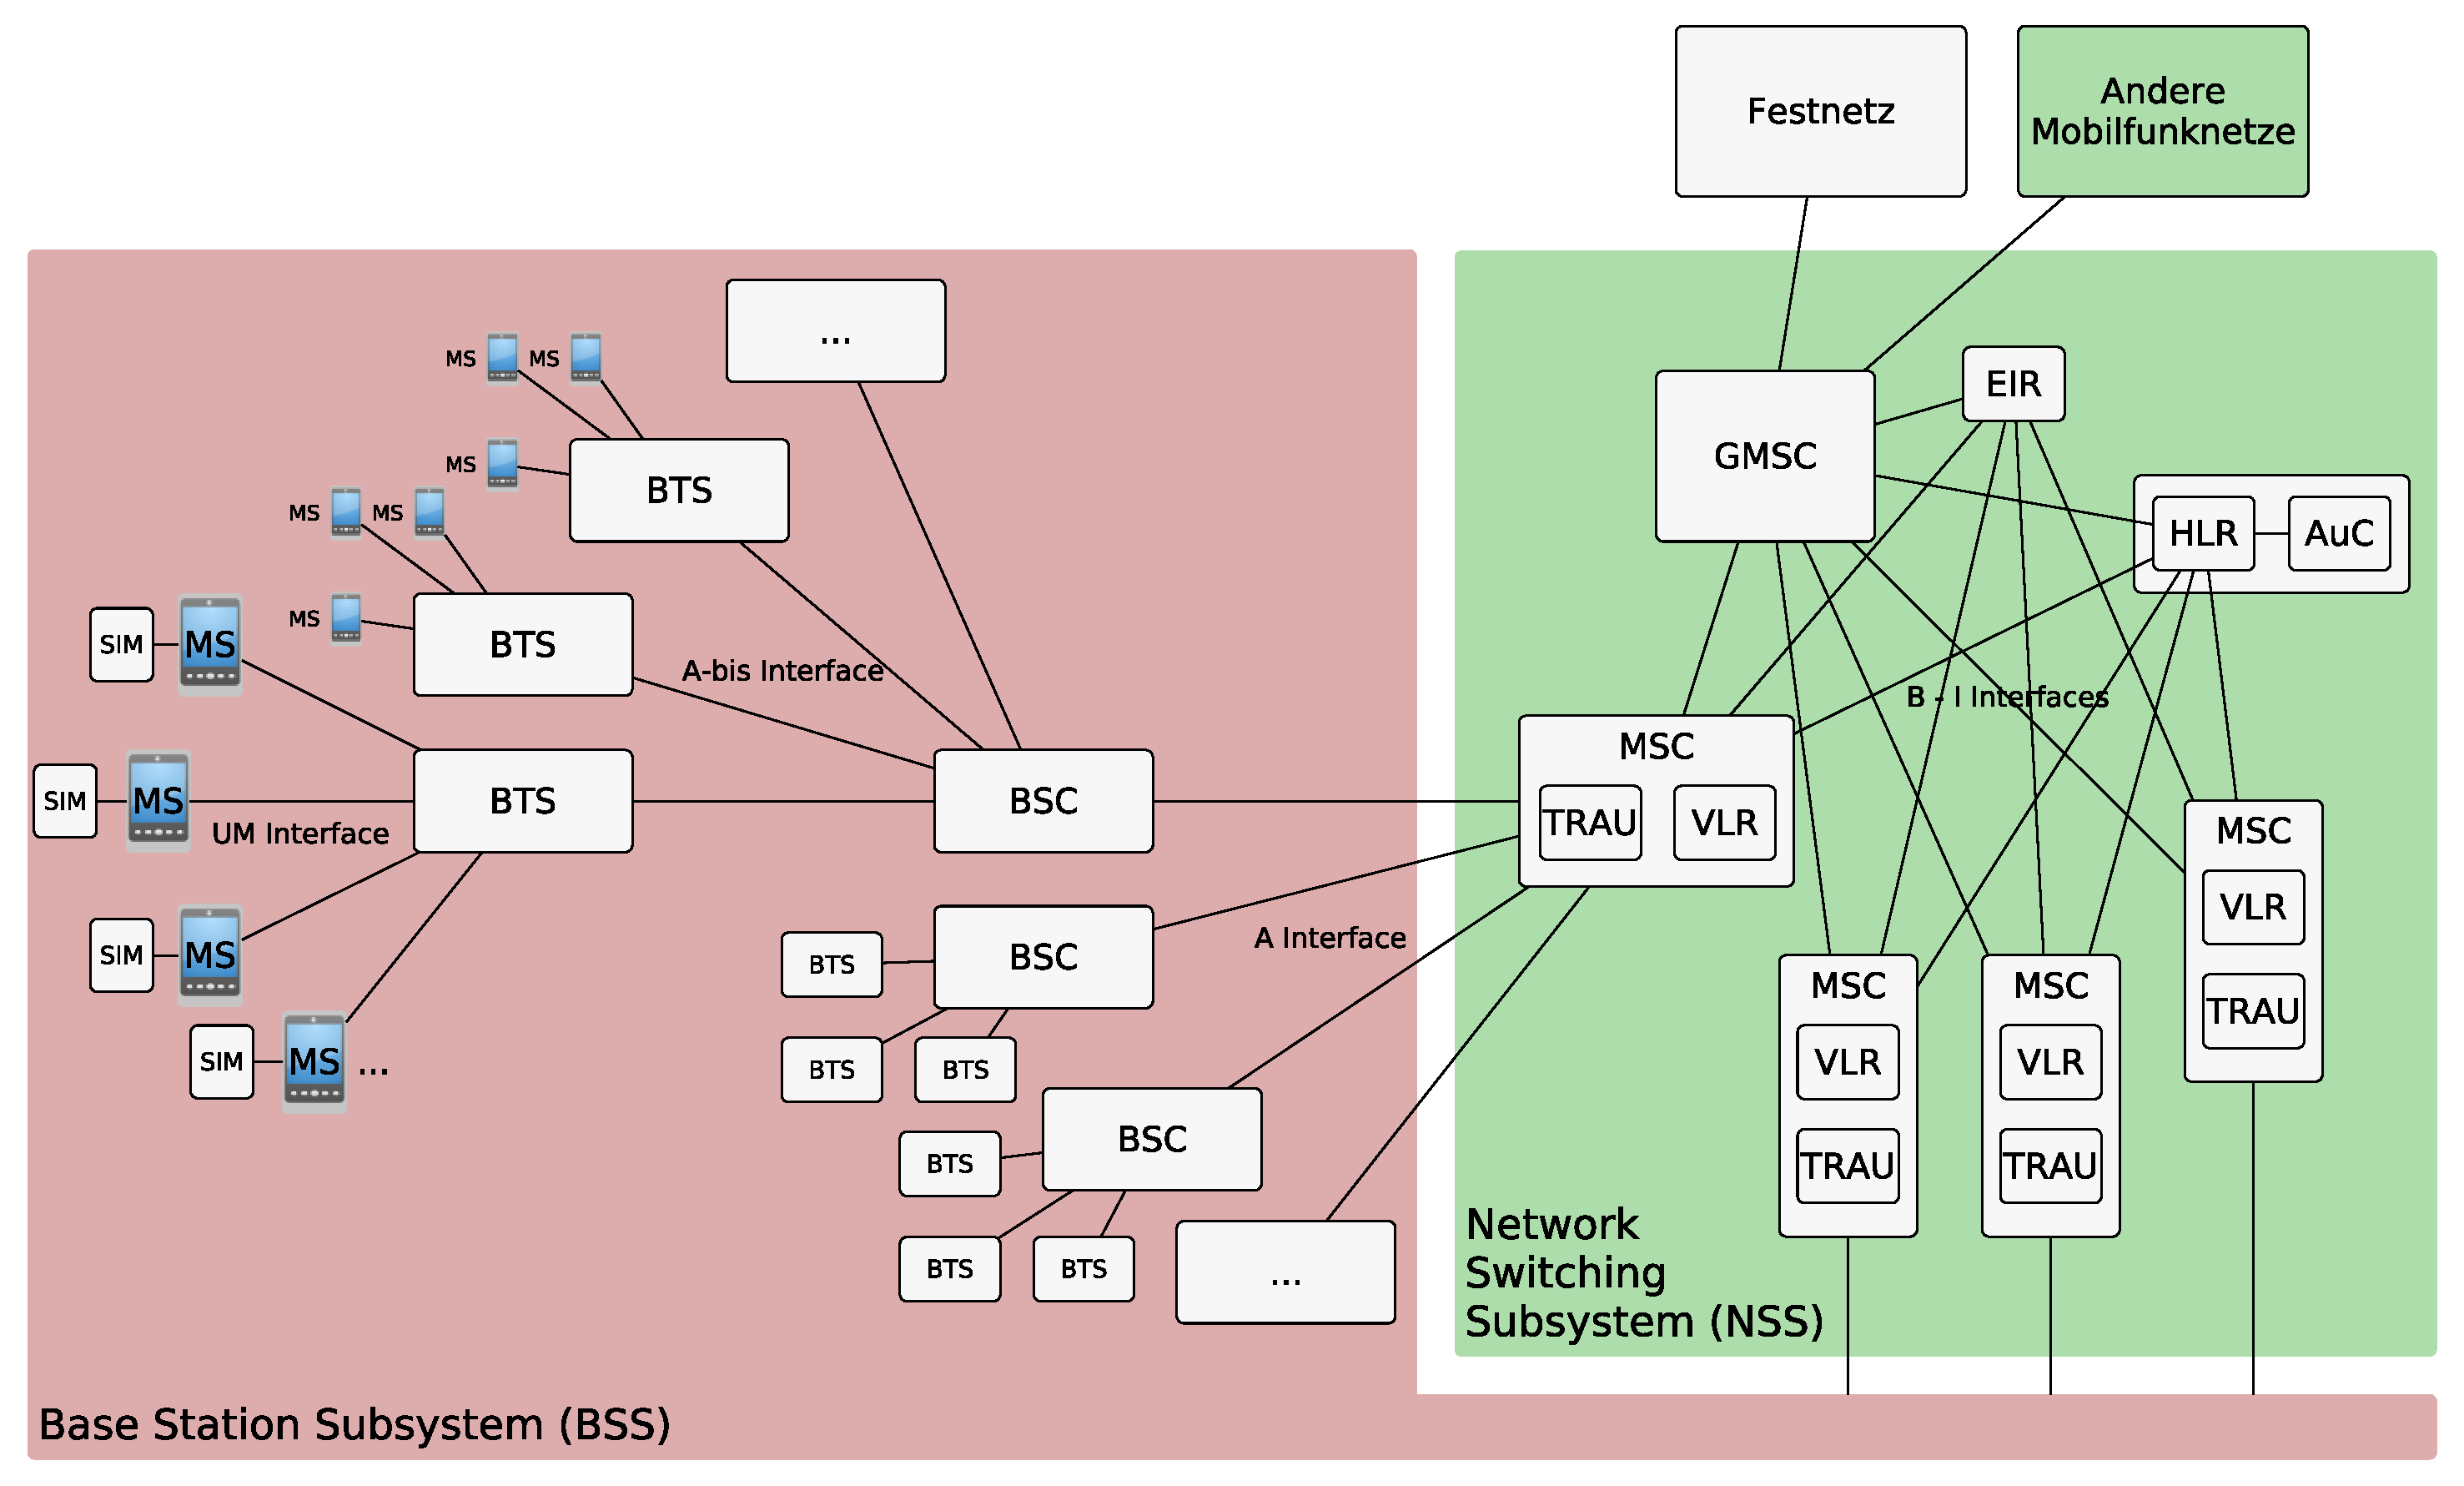
\includegraphics[width=1.0\linewidth]{figures/gsm_network_architecture.pdf}
	  \caption[Die GSM Netzarchitektur]{Die \ac{GSM}-Netzarchitektur, erstellt mit yEd nach \citep{schnabel2003kommunikationstechnik}} \label{fig:gsm-architecture} 
\end{figure}

\begin{description}
\item[\acused{MS}\acs{MS} - \acl{MS}] Die \ac{MS} bezeichnet das mobile Endgerät, das Zugriff auf das Netzwerk erhält. Um die volle Funktionalität des Netzwerks nutzen zu können braucht man eine \acs{SIM}-Karte. Auf ihr sind \ac{IMSI} und geheimer Schlüssel eines Netzteilnehmers gespeichert. Die vom Anbieter zugeteilte \ac{IMSI} identifiziert den Nutzer eindeutig, womit ihm die verwendeten Dienste in Rechnung gestellt werden können. Das \ac{SIM} Modul ist ein Mikrocontroller, der zusammen mit dem \ac{AuC} Zugriff auf den geheimen Schlüssel \acs{Ki} und die Algorithmen \acs{A3} (Authentifizierung) und \acs{A8} (Schlüsselgenerierung) hat. Neben \ac{IMSI} und \acs{Ki} können auch Benutzerdaten wie persönliche Kontakte und der Anrufverlauf gespeichert werden.
\item[\acused{BTS}\acs{BTS} - \acl{BTS}] Die \ac{BTS} kommuniziert über die Funkschnittstelle auf einer oder mehreren zugewiesenen Trägerfrequenzen mit den \acp{MS}. Dabei werden Uplink- und Downlinkfrequenz von einer \ac{ARFCN} definiert. Damit sich benachbarte \ac{BTS} nicht gegenseitig stören, werden ihnen sich nicht überlappende Trägerfrequenzen zugeteilt. Mehrere \acp{MS} können gleichzeitig mit einer \ac{BTS} verbunden sein. 
\item[\acused{BSC}\acs{BSC} - \acl{BSC}] Der \ac{BSC} kann über das Abis Interface auf dem \ac{OML} mehrere \acp{BTS} verwalten und vermittelt Daten vom \ac{NSS} an den zuständigen \ac{BTS}. Nutzdaten von von Mobiltelefonen werden an das \ac{NSS} weitergeleitet.
\item[\acused{MSC}\acs{MSC} - \acl{MSC}] Mehrere \acp{BSC} sind über ein \ac{MSC} mit dem Kernnetzwerk und anderen Netzwerken verbunden. Das \ac{MSC} ist Teil des \ac{SS7} Netzwerks, hat also Zugriff auf alle Komponenten darin. Das \ac{VLR} ist meist direkt im \ac{MSC} integriert.
\item[\acused{HLR}\acs{HLR} - \acl{HLR}] Das \ac{HLR} enthält eine Datenbank mit Informationen aller Netzteilnehmer des Providers sowie das \ac{AuC} mit den Algorithmen \ac{A3} und \ac{A8}. Gespeichert sind Vertragsdetails, Zugriffsberechtigungen auf Netzdienste, aktuelles Guthaben, \acs{Ki}, \ac{MSRN}, aktuelles \ac{VLR} und \ac{MSISDN} zu jeder \ac{IMSI}. Die \ac{MSRN} ermöglicht das Auffinden des Teilnehmers in fremden Netzen beim Roaming. Das aktuelle \ac{VLR} wird für die Lokalisierung im eigenen Netz verwendet. Falls sich beim \ac{LAU} eine \ac{MS} aus dem Zuständigkeitsbereich des \ac{MSC} entfernt, muss im \ac{HLR} die Adresse des \ac{VLR} angepasst werden.
\item[\acused{VLR}\acs{VLR} - \acl{VLR}] Der zeitaufwendige Zugriff des \ac{MSC} auf das \ac{HLR} über das \ac{SS7} wird durch das \ac{VLR} umgangen. Es enthält eine Kopie der Daten des \ac{HLR} und zusätzlich die Felder \ac{TMSI} und \ac{LAI}. Mit dem \ac{LAI} kann der \ac{BSC}, in dessen Zuständigkeitsbereich sich der Teilnehmer gerade befindet, identifiziert werden. Die Teilnehmerdaten sind über \ac{TMSI}, \ac{IMSI} und die \ac{MSRN} indiziert. Die Adresse des \ac{HLR} wird benötigt um Authentifizierungsanfragen an dieses weiterzuleiten.
\item[\acs{Um}-Schnittstelle] (siehe \autoref{hdl:einfuehrung-gsm_schnittstellen_protokolle-um_interface})
Die Funk- oder Radioschnittstelle wird für den Datentransfer zwischen \ac{MS} und \ac{BTS} verwendet. \ac{FDMA} ermöglicht die Kommunikation mit verschiedenen \ac{BTS} und legt die Richtung des Datenflusses (Uplink / Downlink) fest. Mit \ac{TDMA} werden verschiedene Kommunikationskanäle mit einer \ac{BTS} definiert, durch die verschiedene Typen von Signalisierungsinformationen und Daten unterschieden werden können. Übertragene Nachrichten sind kodiert und in der Regel verschlüsselt.
\end{description}

\section{GSM Signalisierungsprotokolle} \label{hdl:einfuehrung-gsm_schnittstellen_protokolle}

Logische Kanäle (siehe \autoref{tab:logical-channels}) können entweder Signalisierungsinformationen oder Nutzdaten übertragen. Wegen der unterschiedlichen Anforderungen werden in \ac{GSM} dafür zwei Protokollstapel definiert - Signaling Plane und User Plane \cite[Kap. 5.2, 5.3]{eberspacher:2008:gsm-architecture}.

\begin{figure}[H]
  \begin{center}
    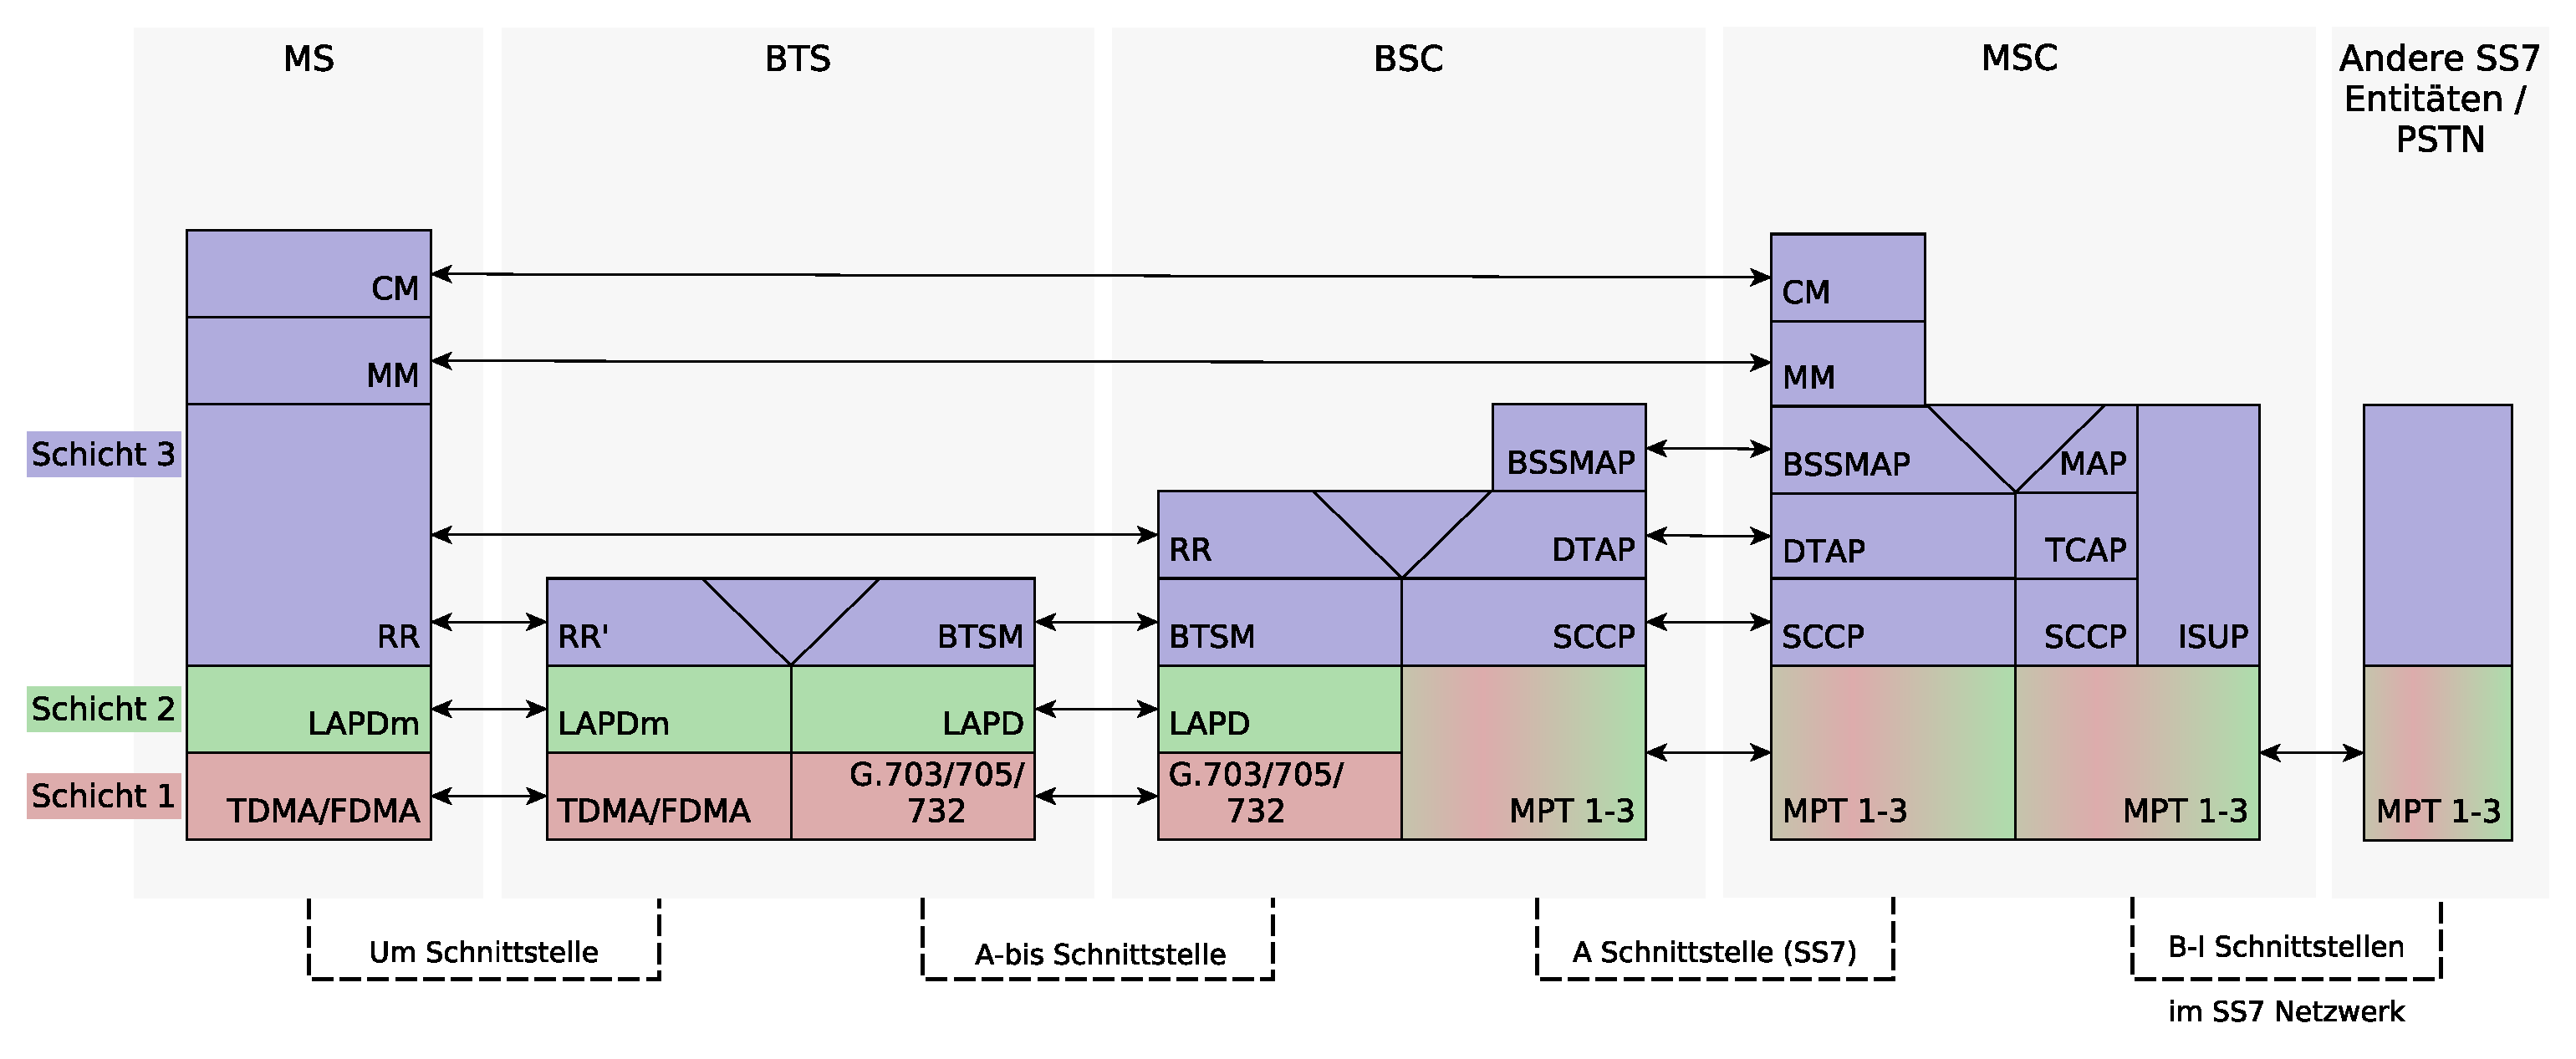
\includegraphics[width=1.0\textwidth]{figures/gsm_protocol_stack.pdf}
  \end{center}
  \caption[Protokollstapel für Signalisierung in GSM]{Protokollstapel für Signalisierung in \ac{GSM}, erstellt mit yEd nach \citep{eberspacher:2008:gsm-architecture}} \label{fig:gsm-protocol-stack} 
\end{figure}

\autoref{fig:gsm-protocol-stack} bietet eine Übersicht über die Signaling Plane, deren Protokollstruktur und Schnittstellen in den folgenden Kapiteln erklärt werden. Hier wegen mangelnder Relevanz nicht erklärte Protokolle und Schnittstellen finden sich im Anhang in \autoref{hdl:a_schnittstellen_protokolle}.

\section{Um Schnittstelle} \label{hdl:einfuehrung-gsm_schnittstellen_protokolle-um_interface}

\acused{Um}

Die Funkschnittstelle zwischen \ac{MS} und \ac{BTS} wird \ac{Um}-Schnittstelle oder auch kurz \ac{Um} genannt. Die Frequenzen für Uplink und Downlink, über die mit einer \ac{BTS} kommuniziert werden kann, werden über die \ac{ARFCN} der \ac{BTS} bestimmt. Auf dem Uplink läuft der Datenfluss Richtung \ac{BTS}, auf dem Downlink Richtung \ac{MS}. Da die Übertragung über die Funkschnittstelle fehlerbehaftet ist, müssen für eine zuverlässige Verbindung Fehlerkorrekturmechanismen implementiert sein.

Das Übertragungsprotokoll der physikalischen Schicht basiert auf einer Kombination aus \ac{FDMA} und \ac{TDMA} (siehe \autoref{hdl:a_tdma_fdma}). Durch \ac{FDMA} wird das verfügbare Frequenzband in verschiedene Trägerfrequenzen unterteilt. Mit \ac{TDMA} werden auf einer Trägerfrequenz acht Zeitschlitze definiert und physikalischen Kanälen zugeteilt. Einem physikalischen Kanal wird durch Multiframes wiederum eine sich wiederholende Sequenz logischer Kanäle zugewiesen. Logische Kanäle bieten verschiedene Funktionen an. Auf \acp{TCH} werden zum Beispiel Sprachdaten, auf \acp{BCCH} Broadcast Signalisierungsdaten und auf \acp{CCCH} Signalisierungsdaten für einzelne Teilnehmer übertragen.

Im Zeitschlitz eines physikalischen Kanals kann genau die Datenmenge eines Bursts übertragen werden. In \autoref{fig:normal_burst} ist der Aufbau eines normalen Bursts dargestellt. Normale Burst werden in \ac{GSM} sowohl für die Übertragung von Nutzdaten auf \acp{TCH}, als auch für die Übertragung von Signalisierungsnachrichten auf \ac{SDCCH}, \ac{SACCH}, \ac{FACCH} und weiteren verwendet. Wie man in der Grafik sehen kann, trägt jeder Burst zwei 57 Bit Datenblöcke auf einmal. Traingssequenz, vorderer und hinterer Tail sind für die Funkübertragung relevant und für diese Arbeit nicht von Bedeutung. Auf die Stealing Flags wird im folgenden Abschnitt eingegangen. Der Aufbau verschiedener Bursttypen kann in \citepauthor[Kap. 5.2.3]{3gpp:05.02} nachgelesen werden.

\begin{figure}[H]
  \begin{center}
    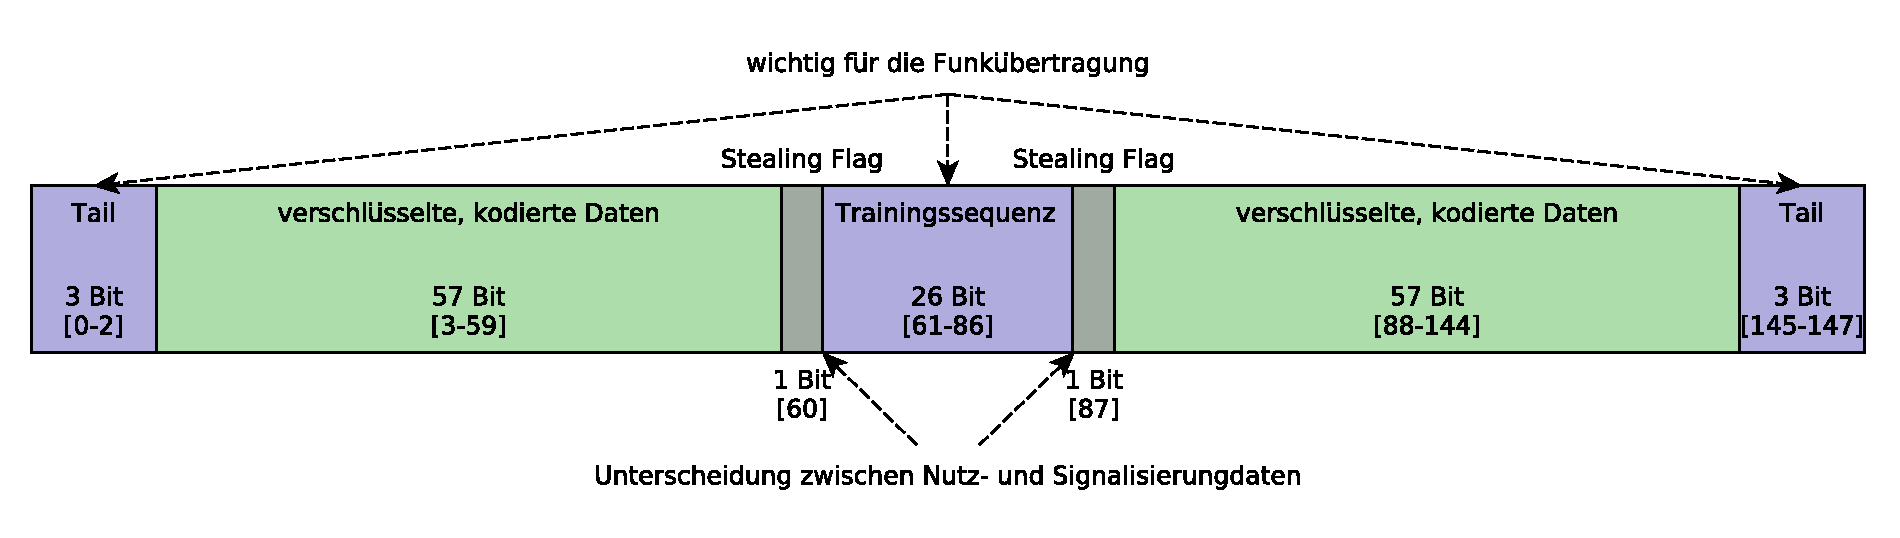
\includegraphics[width=1.0\textwidth]{figures/normal_burst.pdf}
  \end{center}
  \caption[Der Aufbau eines normalen Bursts]{Der Aufbau eines normalen Bursts, erstellt mit yEd nach \citepauthor[Kap. 5.2.3]{3gpp:05.02}} \label{fig:normal_burst} 
\end{figure}

\subsection{Logische Kanäle -- GSM-Multiframe}\label{hdl:logical-channels}

Physikalischen Kanälen können verschiedene Sequenzen logischer Kanäle zugeordnet werden\citepauthor[Kap. 6]{3gpp:04.03}.

Es wird ein sich wiederholendes Multiframe definiert, welches sich auf Signalisierungskanälen nach 51 Frames und auf Datenkanälen nach 26 Frames wiederholt. Die Struktur des Multiframes, also die Sequenz seiner logischen Kanäle, ordnet damit einer Nachricht, über ihre \ac{FN}, genau einem logischen Kanal zu. Durch die unterschiedliche Größe der Multiframes für \ac{TCH}, \ac{BCCH} und \ac{CCCH} beginnen diese erst nach ihrem gemeinsamen Vielfachen ($26 \cdot 51$ Frames) wieder zusammen von vorne -- einem Superframe. Aufgrund der begrenzten Größe der \ac{FN} wird ein Hyperframe von 2048 Superframes definiert, nach der die \ac{FN} wieder bei 0 beginnt \citepauthor[Kap. 6]{3gpp:05.02}. Die \ac{FN} wiederholt sich also alle 3 Stunden, 28 Minuten und 53.76 Sekunden. 

\begin{figure}[H]
  \begin{center}
    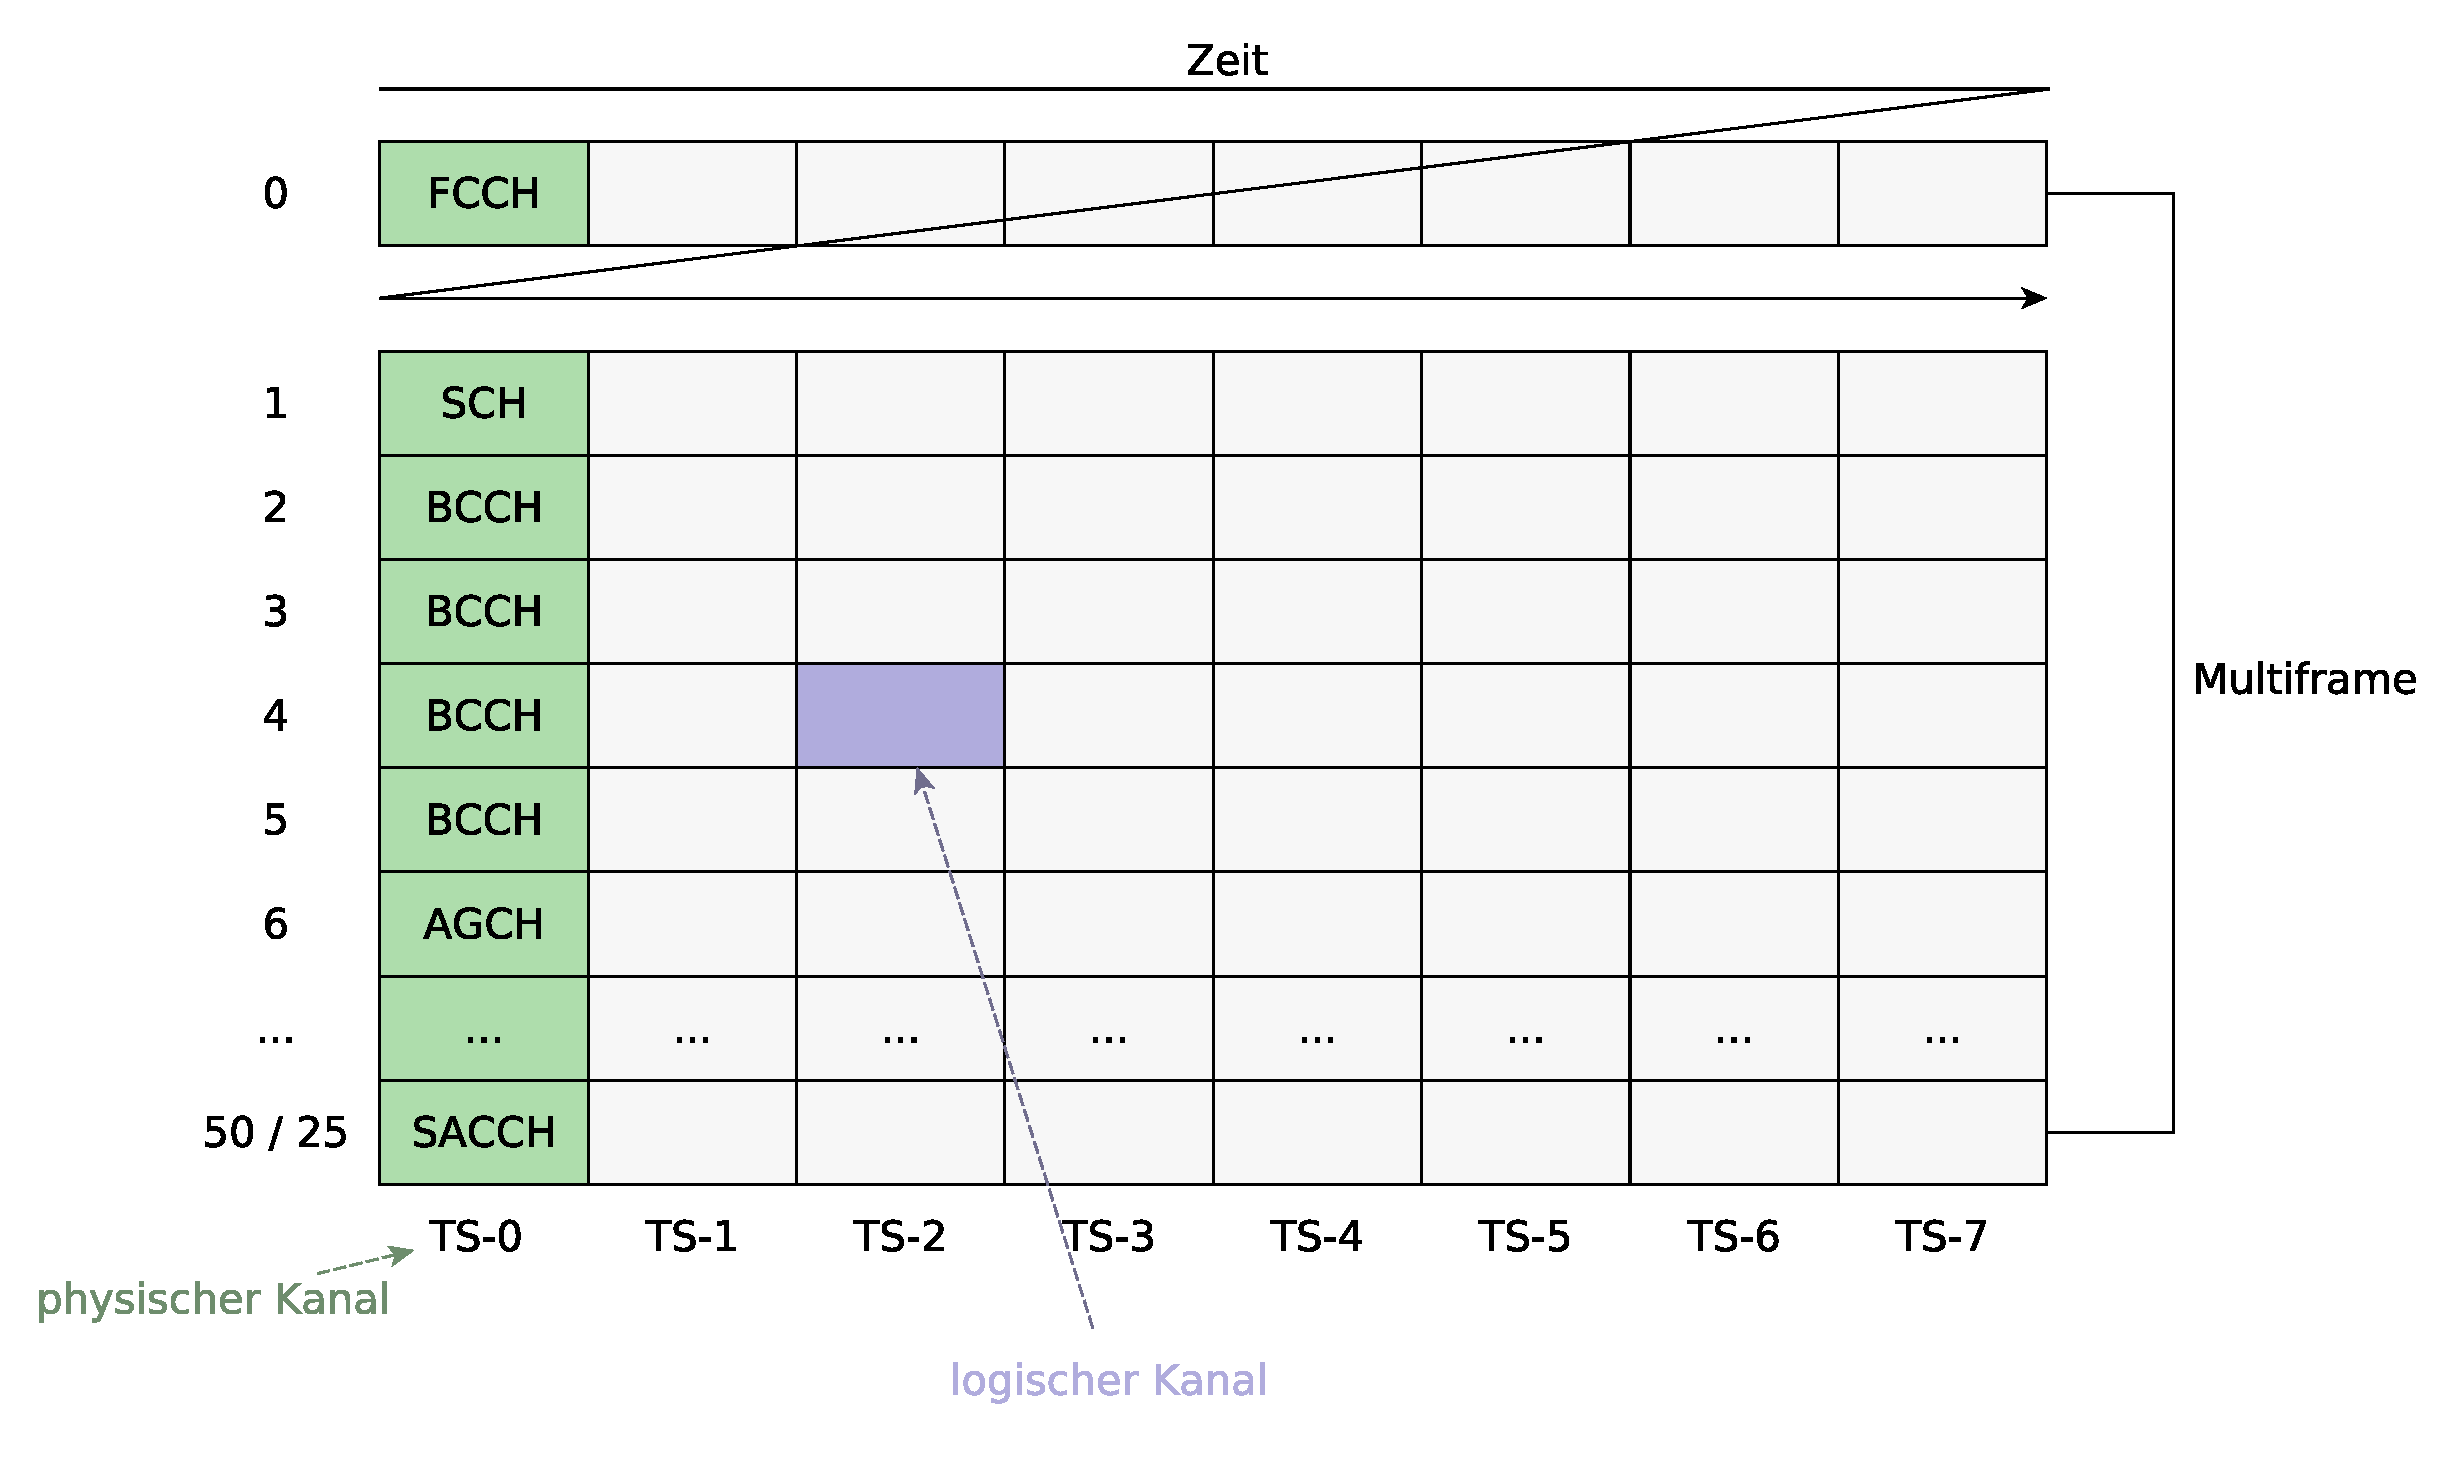
\includegraphics[width=1.0\textwidth]{figures/gsm_multiframe.pdf}
  \end{center}
  \caption[Die GSM Multiframe Struktur]{Die \ac{GSM} Multiframe Struktur, erstellt mit yEd nach \citep[Kap. 1.7.3]{sauter:2011:grundkurs-mobile}} \label{fig:gsm-multiframe} 
\end{figure}

In \ac{GSM} wird jedem physikalischen Kanal ein Multiframe zugeordnet. Das Multiframe, das für die Bestimmung des logischen Kanals einer Nachricht angewendet wird, ist also durch den Zeitschlitz bestimmt, auf dem die Nachricht übertragen wurde. Aus der \ac{FN}, mit der die Nachricht empfangen wurde, wird das Offset im Multiframe berechnet und ihr damit ein logischer Kanal zugeordnet. Die \ac{FN} und der physikalische Kanal bestimmen also eindeutig den logischen Kanal einer Nachricht. \autoref{tab:logical-channels} gibt eine Übersicht über die logischen Kanäle und ihre Funktionen.

Kanäle vom Typ \ac{BCCH}, \ac{CCCH} und \ac{DCCH} übertragen Signalisierungsinformationen und sind Teil der Signaling Plane. Der \ac{TCH} überträgt ausschließlich Sprachdaten und wird der User Plane zugeordnet. Der \ac{SDCCH} wird für Signalisierung und im Fall von \ac{SMS} Nachrichten auch für Nutzdaten verwendet, weshalb durch Multiplexing zwischen User und Signaling Plane unterschieden wird. Für das Multiplexing ist das \ac{SAPI} Feld des \ac{LAPDm} Headers zuständig (siehe \autoref{hdl:einfuehrung-gsm_schnittstellen_protokolle-um_interface-layer2}).

\begin{table}[H]
\begin{adjustbox}{width={1.00\textwidth}, center}
\begin{tabular}{|l|l|l|l|}
\rowcolor[HTML]{F7F7F7} 
\hline
\textbf{Name} & \textbf{Beschreibung}                 	& \textbf{Richtung} & \textbf{Typ} 	\\ \hline
\acs{BCCH}          & \acl{BCCH}              			& Downlink          & Broadcast    		\\ \hline
\acs{SCH}           & \acl{SCH}               			& Downlink          & Broadcast   		\\ \hline
\acs{FCCH}          & \acl{FCCH}        			  	& Downlink          & Broadcast    		\\ \hline
\acs{AGCH}          & \acl{AGCH}                  		& Downlink          & Common Control       		\\ \hline
\acs{PCH}           & \acl{PCH}                         & Downlink          & Common Control       		\\ \hline
\acs{RACH}          & \acl{RACH}                 		& Uplink            & Common Control       		\\ \hline
\acs{FACCH}         & \acl{FACCH}       				& Bidirektional     & Dedicated Control    		\\ \hline
\acs{SACCH}         & \acl{SACCH}       				& Bidirektional     & Dedicated Control    		\\ \hline
\acs{SDCCH}         & \acl{SDCCH} 						& Bidirektional     & Dedicated Control    		\\ \hline
\acs{TCH}           & \acl{TCH}                       	& Bidirektional     & Nutzdatenkanal  \\ \hline
\end{tabular}
\end{adjustbox}
\caption{Die logischen Kanäle der Funkschnittstelle}\label{tab:logical-channels}
\end{table}
\acused{BCCH}\acused{SCH}\acused{FCCH}\acused{AGCH}\acused{PCH}\acused{RACH}\acused{FACCH}\acused{SACCH}\acused{SDCCH}\acused{TCH}

\textbf{\acfp{BCCH}} werden für Nachrichten von der \ac{BTS} an alle sich im Empfangsbereich befindenden \acp{MS} verwendet. Es gibt sie deshalb nur im Downlink. \citepauthor[Kap. 4.1.1]{3gpp:04.03}
\begin{itemize}
\item \textbf{\ac{BCCH}}: Auf dem \ac{BCCH} werden über die \ac{SI} Nachrichten regelmäßig Konfiguration und Parameter des Netzwerks verschickt. Davon gibt es insgesamt 9, von denen aber nur \ac{SI}-1 bis \ac{SI}-4 auf dem \ac{BCCH} übertragen werden.
\item \textbf{\ac{SCH}}: Die auf diesem Kanal gesendeten Bursts ermöglichen es Endgeräten, sich mit der Multiframe-Struktur der \ac{BTS} zu synchronisieren. Damit das \ac{MS} den Burst dekodieren kann, obwohl es zu diesem Zeitpunkt die Entfernung und damit den genauen Anfang des empfangenen Bursts nicht kennt, haben die Synchronisation-Bursts ein spezielles Format.
\item \textbf{\ac{FCCH}}: Dieser Kanal dient zur Kalibrierung des Transceivers der \ac{MS} und definiert den Anfang des Multiframes.
\end{itemize}

Auf den \textbf{\acfp{CCCH}} werden Signalisierungsinformationen ausgetauscht, mit denen dedizierte bidirektionale Kanäle beantragt und vergeben werden können. Die \acp{CCCH} werden von mehreren \acp{MS} verwendet. \citepauthor[Kap. 4.1.2]{3gpp:04.03}
\begin{itemize}
\item \textbf{\ac{RACH}}: Auf dem einzigen Kanal den es nur im Uplink gibt, können \acp{MS} mit einem sogenannten "`Channel Request"' vom Netzwerk einen dedizierten Kanal anfordern.
\item \textbf{\ac{AGCH}}: Der \ac{AGCH} wird verwendet, um einer \ac{MS} nach einem Channel-Request einen dedizierten Kanal zuzuweisen.
\item \textbf{\ac{PCH}}: Auf dem \ac{PCH} werden \acp{MS} im Empfangsbereich einer Basisstation über eingehende Anrufe und \ac{SMS} informiert.
\end{itemize} 

Die bidirektionalen \textbf{\acfp{DCCH}} sind einer dedizierten Verbindung zwischen \ac{BTS} und \ac{MS} zugeordnet. Um sie vor Zugriff von anderen zu schützen wird der Datentransfer auf \acp{DCCH} in der Regel verschlüsselt. \citepauthor[Kap. 4.1.3]{3gpp:04.03}
\begin{itemize}
\item \textbf{\ac{FACCH}}: Der \ac{FACCH} ist ein Signalisierungskanal, der auf einem \ac{TCH} übertragen wird. Er wird für dringende Signalisierungsnachrichten verwendet, wobei die Nutzdaten des Bursts durch Signalisierungsinformationen ersetzt werden. Ob der \ac{TCH}-Burst vom \ac{FACCH} gestohlen wurde, wird durch Setzen eines "`Stealing Flags"' gekennzeichnet. Der Qualitätsverlust der Sprachübertragung durch die fehlenden Nutzdaten ist nicht hörbar.
\item \textbf{\ac{SACCH}}: Der \ac{SACCH} wird im Uplink für die Übertragung von Messdaten, wie der Signalstärke benachbarter \ac{BTS}, verwendet. Im Downlink erhält die \ac{MS} Befehle zu Leistungsregelung von der \ac{BTS}. 
\item \textbf{\ac{SDCCH}}: Der \ac{SDCCH} wird für die Signalisierung bei der Nutzung von Netzdiensten verwendet, zum Beispiel für den Aufbau eines Gesprächs, das Einrichten einer verschlüsselten Verbindung, Identitätsabfragen, Authentifizierung und "`Location Updates"'. Freie Kapazitäten werden für den Empfang und Versand von \ac{SMS} Nachrichten benutzt. In diesem Fall dient er auch der Übertragung von Nutzdaten.
\end{itemize}

Der \textbf{\ac{TCH}} ist ein bidirektionaler, dedizierter Nutzdatenkanal, über den entweder Sprachdaten oder leitungsvermittelte Datendienste übertragen werden.

\subsection{Service Access Point}\label{hdl:sap}

Ein \ac{SAP} ist eine interne Schnittstelle zwischen Protokollschichten. Die Kommunikation zwischen den Schichten basiert dabei, wie in \ac{GSM} üblich, auf Primitives. Es gibt folgende Typen von Primitives \citepauthor{3gpp:04.04}:

\begin{itemize}
\item \textbf{\ac{IND}}: Layer 1 $\rightarrow$ Layer 2+\\
Benachrichtigung höherer Schichten über Vorkommnisse auf dieser Schicht -- wie zum Beispiel eingehende Daten.
\item \textbf{\ac{REQ}}: Layer 1 $\leftarrow$ Layer 2+\\
Höhere Schichten können damit vom \ac{SAP} angebotene Dienste nutzen.
\item \textbf{\ac{RES_proto}}: Layer 1 $\leftarrow$ Layer 2+\\
Bestätigung des Empfangs einer Indication.
\item \textbf{\ac{CON}}: Layer 1 $\rightarrow$ Layer 2+\\
Antwort auf Response nach erfolgreich abgearbeiteter Routine.
\end{itemize}

Folgende Abbildung aus \citetauthor{3gpp:04.04} zeigt die Schnittstellen der physikalischen Schicht in \ac{GSM} zu anderen Protokollschichten. Die physikalische Schicht bietet \ac{SAP}-Schnittstellen zur Datensicherungsschicht und dem Schicht 3 zugeordneten \ac{RR}-Management, die über PH-Primitives und MPH-Primitives angesprochen werden können.

\begin{figure}[H]
  \begin{center}
    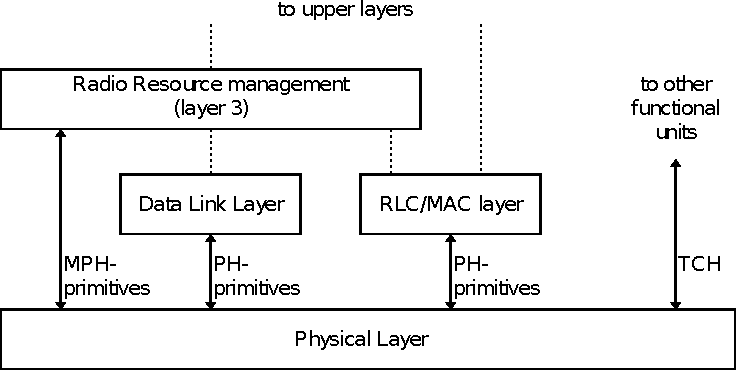
\includegraphics[width=0.8\textwidth]{figures/0404_fig_21.pdf}
  \end{center}
  \caption[Die Schnittstellen der physikalischen Schicht]{Die Schnittstellen der physikalischen Schicht, aus \citepauthor[Abb. 2.1]{3gpp:04.04}} \label{fig:interface-physical-layer} 
\end{figure}

Die logischen Kanäle definieren im Fall der physikalischen Schicht unterschiedliche \acp{SAP} zu \ac{LAPDm}, wie in \autoref{fig:sap-logical-channels} zu sehen ist.

\begin{figure}[H]
  \begin{center}
    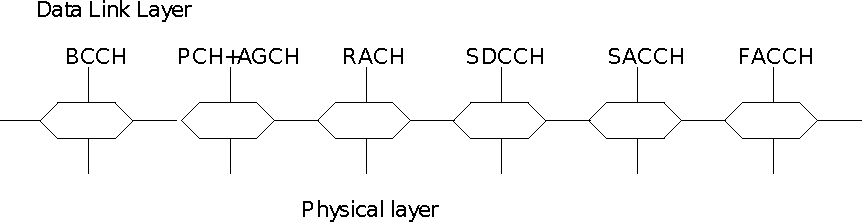
\includegraphics[width=0.95\textwidth]{figures/0404_fig_23.pdf}
  \end{center}
  \caption[SAPs der physikalischen Schicht zur Sicherungsschicht ]{\acp{SAP} der physikalischen Schicht zur Sicherungsschicht, aus \citepauthor[Abb. 3.2]{3gpp:04.04}} \label{fig:sap-logical-channels} 
\end{figure}


\subsection{Link Access Protocol Dm-Channel}
\label{hdl:einfuehrung-gsm_schnittstellen_protokolle-um_interface-layer2}

Die Aufgabe des in \citetauthor{3gpp:04.05} und \citetauthor{3gpp:04.06} spezifizierten \ac{LAPDm}-Protokolls der Datensicherungsschicht ist der Aufbau einer zuverlässigen Verbindung zwischen \ac{MS} und \ac{BTS}. Für die zuverlässige Übertragung von Daten stellt es einen \ac{SAP} für Schicht 3 zur Verfügung, selbst greift es auf die von der physikalischen Schicht angebotenen \acp{SAP} der logischen Kanäle zu (siehe \autoref{fig:sap-logical-channels}). Das zwischen \ac{MS} und \ac{BTS} terminierende Protokoll wurde in großen Teilen aus der \ac{ISDN}-Spezifikation des Protokolls \ac{LAPD} übernommen und an die Anforderungen der Funkschnittstelle angepasst. 

Das Protokoll soll mehrere Einheiten von physikalischer Schicht und Schicht 3 unterstützen, sowie die Signalisierung auf \ac{BCCH}, \ac{CCCH} und \ac{DCCH}. In \citetauthor[Kap. 3.1]{3gpp:04.05} wird sein Funktionsumfang wie folgt beschrieben:

\begin{itemize}
\item Unterstützung einer oder mehrerer Schicht 3 Datenverbindungen, die durch einen \ac{DLCI} identifiziert werden.
\item Unterscheidung verschiedener Nachrichtentypen.
\item Transparente Nachrichtenübertragung zwischen Schicht 3 Einheiten.
\item Sicherstellen der korrekten Reihenfolge der Nachrichten (Ablaufsteuerung).
\item Anpassen der Datenrate an Eigenschaften der physikalischen Schicht (Flusskontrolle).
\item Benachrichtigung von Schicht 3 Einheiten über nicht behebbare Fehler. 
\end{itemize}

\ac{LAPDm} bietet Schicht 3 zwei verschiedenen Übertragungsoperationen an. Die unzuverlässige "`unacknowledged operation"' und die zuverlässige "`acknowledged operation"'. Auf \ac{BCCH} und \ac{CCCH} ist nur die unzuverlässige Operation verfügbar, auf \ac{DCCH} können beide benutzt werden. Mit den beiden Übertragungstypen realisiert \ac{LAPDm} die Dienste "`Unacknowledged Information Transfer"' für unzuverlässige und "`Acknowledged Multiple Frame Information Transfer"' für zuverlässige Datenverbindungen.

\subsubsection*{Unacknowledged Information Transfer}

Von Schicht 2 wird weder die korrekte Reihenfolge verifiziert, noch dass eine gesendete Nachricht beim Empfänger angekommen ist \citepauthor[Kap. 4.2.4]{3gpp:04.05}. Nachrichten werden als \ac{UI}-Frames übertragen. 

\subsubsection*{Acknowledged Multiple Frame Information Transfer}
\acused{N(R)}\acused{N(S)}\acused{RRm}

Durch Kontrollmechanismen von Schicht 2 wird sichergestellt, dass übertragene Daten in der richtigen Reihenfolge beim Empfänger ankommen \citepauthor[Kap. 4.2.5]{3gpp:04.05}. Auf beiden Seiten werden jeweils die Nummern \ac{N(R)} empfangener und \ac{N(S)} gesendeter Nachrichten gepflegt. Die übertragenen \ac{I}-Frames enthalten diese beiden Zähler. Durch Synchronisation der empfangenen Nummern mit den eigenen kann so festgestellt werden, ob Daten verloren gegangen sind oder die Reihenfolge nicht mehr stimmt. Mit einer \ac{REJ} Nachricht kann eine fehlerhaft empfangene Nachricht abgewiesen werden, mit Receive-Ready (\acs{RRm})-Nachrichten wird der Gegenseite mitgeteilt, welche Nachricht sie als nächstes schicken soll. Ein \ac{RRm} enthält dazu die Nummer $\ac{N(R)} + 1$ und bestätigt gleichzeitig den Empfang aller Nachrichten bis zu dieser. Sollte die Datensicherungsschicht keine Möglichkeit haben eine zuverlässige Verbindung zu gewährleisten, wird ein Fehler an Schicht 3 gemeldet. Mit einer \ac{SABM}-Nachricht signalisiert Schicht 2 ihrer Gegenseite, dass in den zuverlässigen Übertragungsmodus gewechselt werden soll. Diese bestätigt den Wechsel mit einer \ac{UA}-Nachricht. Mit einem \ac{DISC} kann von beiden Seiten die Verbindung wieder beendet und in den unzuverlässigen Modus gewechselt werden \citepauthor[Kap. 5.4]{3gpp:04.06}.

\subsubsection*{Aufbau eines LAPDm-Frames} \label{hdl:lapdm-format}

Für \ac{LAPDm}-Nachrichten auf verschiedenen logischen Kanälen werden auch verschiedene Formate definiert. Da für die Masterarbeit nur \ac{LAPDm} Nachrichten auf \ac{DCCH} untersucht werden, wird hier nur auf das "`Frame Format A"' eingegangen. Dieses ist, wie auch die anderen Formate, in \citetauthor[Kap. 2]{3gpp:04.06} definiert.

\begin{figure}[H]
	\centering 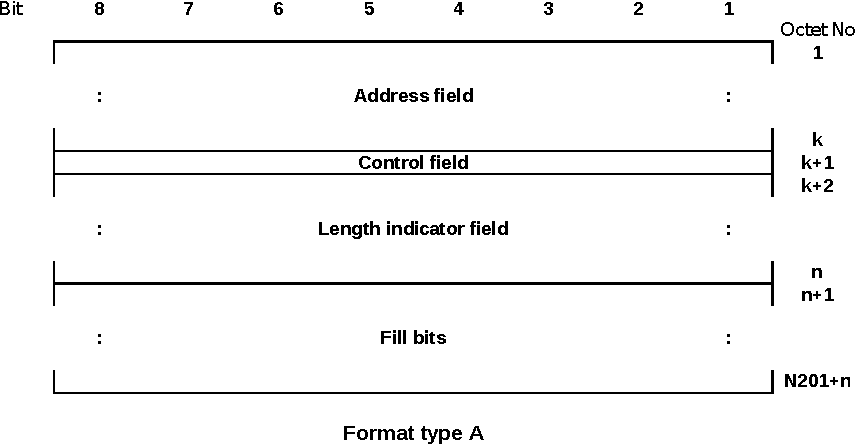
\includegraphics[width=0.9\linewidth]{figures/0406_fig_1_pt_1.pdf}
	\caption[Das LAPDm Format A]{Das \ac{LAPDm} Format A, aus \citep[Abb. 1, Teil 1]{3gpp:04.06}} \label{fig:lapdm-format-a}
\end{figure}

Obige Abbildung zeigt die \ac{LAPDm}-Nachricht im Format A. Sie setzt sich aus je einem Byte (Oktett) für Adressierungs-, Kontroll- und Längeninformationen und N201 Bytes an Nutzdaten zusammen. Die Größe von N201 wird in \citetauthor[Kap. 5.8.3]{3gpp:04.06} für \ac{FACCH} und \ac{SDCCH} als 20 definiert, damit ist die gesamte Nachricht 23 Bytes oder 184 Bit lang. 

\begin{figure}[H]
	\centering 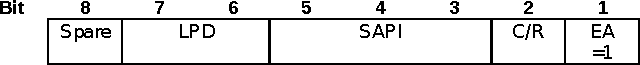
\includegraphics[width=0.8\linewidth]{figures/0406_fig_4.pdf}
	\caption[Das LAPDm Addressierungsfeld]{Das \ac{LAPDm} Addressierungsfeld, aus \citep[Abb. 4]{3gpp:04.06}} \label{fig:lapdm-format-addr}
\end{figure}

Das oben gezeigte Adressierungsfeld liefert Informationen über den Sender und Empfänger der Nachricht. Das \ac{EA} sagt aus, ob dies das letzte Byte des Adressierungsfeldes ist oder noch weitere folgen. Es wird benötigt, da das Adressierungsfeld auch mehrere Bytes lang sein kann. Das \ac{C/R} definiert ob es sich um einen Befehl (Command) oder die Antwort auf diesen (Response) handelt. Die \ac{SAPI} entspricht dem \ac{DLCI} und definiert die Schicht 3 Datenverbindung, für die die Nachricht bestimmt ist. Das \ac{LPD}-Feld identifiziert das verwendete Schicht 2 Protokoll und ist in \ac{LAPDm} immer 0.

\begin{figure}[H]
	\centering 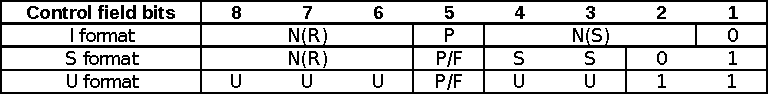
\includegraphics[width=0.8\linewidth]{figures/0406_tab_3.pdf}
	\caption[Das LAPDm Kontrollfeld]{Das \ac{LAPDm} Kontrollfeld, aus \citep[Tabelle 3]{3gpp:04.06}} \label{fig:lapdm-format-ctl}
\end{figure}

Der oben gezeigte Aufbau des Kontrollfelds hängt mit dem verwendeten Nachrichtenformat zusammen. Beim nummerierten \ac{I}-Format (Bit[1] == 0) gibt es die Nummer der letzten korrekt empfangenen Nachricht \ac{N(R)} und die Nummer der zuletzt gesendeten Nachricht \ac{N(S)}. Das \ac{S} (Bit[1,2] == 10) benötigt die Nummer \ac{N(R)} der erwarteten nächsten Nachricht und zwei S-Bits, die die verwendete Supervisory Funktion (zum Beispiel \ac{RRm}) bestimmen. Das \ac{U} (Bit[1,2] == 11) ist nicht durchnummeriert und benutzt alle U-Bits für die Bestimmung der verwendeten Unnumbered Funktion (zum Beispiel \ac{SABM}). Das \ac{P/F} definiert bei einem Command, ob man eine Antwort der Gegenseite möchte und bei einer Response, ob es sich um eine Antwort auf einen "`Poll"' der Gegenseite handelt.

\begin{figure}[H]
	\centering 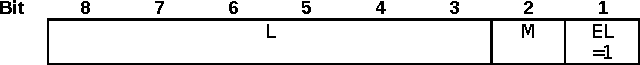
\includegraphics[width=0.9\linewidth]{figures/0406_fig_5.pdf}
	\caption[Das LAPDm Längeninformationsfeld]{Das \ac{LAPDm} Längeninformationsfeld, aus \citep[Abb. 5]{3gpp:04.06}} \label{fig:lapdm-format-len}
\end{figure}

Das \ac{EL} der oben gezeigten Längeninformation sagt aus, ob es sich bei diesem um das letzte Byte handelt (siehe \ac{EA} im Adressierungsfeld). Das \ac{M} zeigt an, ob sich die übertragene Signalisierungsnachricht aus mehr als dieser \ac{LAPDm}-Nachricht zusammensetzt. Das wird benötigt, wenn mehr als 160 Bit an Signalisierungsinformationen übertragen werden müssen, da diese nicht mehr in eine einzelne \ac{LAPDm}-Nachricht passen. Der \ac{L} gibt die Länge der Nutzdaten in dieser Nachricht an. Alle Daten nach der definierten Länge enthalten keine nützlichen Information mehr und werden in der Regel mit \texttt{0x2b} aufgefüllt.

\section{Schicht 3 Protokolle}

Die Protokollebene 3 besteht in \ac{GSM} aus \acf{RR}, \acf{MM} und \acf{CM}, die verschiedene Aufgaben übernehmen. Ein Teil des \ac{RR}-Protokolls fällt in den Aufgabenbereich der \ac{BTS} und wird von dieser bearbeitet, der Rest wird transparent an den \ac{BSC} weitergeleitet. \ac{MM} und \ac{CM} werden weder von \ac{BTS} noch \ac{BSC} bearbeitet und den Protokollen zugewiesene Nachrichten zwischen \ac{MS} und \ac{MSC} ausgetauscht. Der für die Funkschnittstelle relevante Teil der Protokolle ist in \citetauthor{3gpp:04.18} spezifiziert, der Rest findet sich in \citetauthor{3gpp:24.008} und \citetauthor{3gpp:23.108}.

\begin{figure}[H]
	\centering 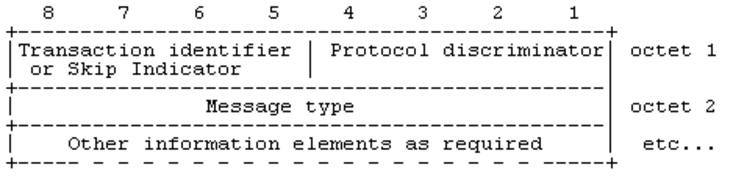
\includegraphics[width=0.9\linewidth]{figures/24008_fig_10-1.pdf}
	\caption[Der gemeinsame Header der Schicht 3 Protokolle]{Der gemeinsame Header der Schicht 3 Protokolle, aus \citep[Abb. 10.1]{3gpp:24.008}} \label{fig:l3-common-hdr}
\end{figure}

Die Protokolle teilen sich den in \autoref{fig:l3-common-hdr} gezeigten, gemeinsamen Header \citep[11.2.3.1]{3gpp:24.007}. Bit 1 bis 4 werden einem Protokolldiskriminator zugeordnet und ermöglichen die Unterscheidung der verschiedenen Schicht 3 Protokolle. Die für die Arbeit relevanten Werte für diesen sind in \autoref{tab:l3-prot-disc-values} aufgeführt. Bit 5 bis 8 kann entweder unbenutzt bleiben und übersprungen werden ("`Skip Indicator"') oder für die Zuordnung der Nachricht zu einer von bis zu 16 Transaktionen oder Verbindungen (\ac{TI}) verwendet werden. Das zweite Byte ist für den Typ der übertragenen Nachricht reserviert ("`Message Type"'), von denen die Schicht 3 Protokolle verschiedene spezifizieren können. 

\begin{table}[H]
\centering
\begin{tabular}{|l|l|}
\hline
Bits 4 3 2 1 & Protokoll                 \\ \hline
0 0 1 1      & Call Control              \\ \hline
0 1 0 1      & Mobility Management       \\ \hline
0 1 1 0      & Radio Resource Management \\ \hline
1 0 0 1      & SMS                       \\ \hline
\end{tabular}
\caption[Werte des Schicht 3 Protokolldiskriminators]{Werte des Schicht 3 Protokolldiskriminators, nach \citep[Tabelle 11.2]{3gpp:24.007}}
\label{tab:l3-prot-disc-values}
\end{table}

Die Informationsfelder des Schicht 3 Headers sind im \ac{TLV} Format angegeben. Der "`Type"' ist der \ac{IEI} des Informationselements, "`Length"' seine Länge und "`Value"' sein Wert. Damit ist es möglich, optionale Informationselemente dynamischer Länge aneinanderzureihen. Ist die Position des Feldes festgelegt, muss T nicht mit angegeben werden. Ist die Länge festgelegt, muss L nicht angegeben werden. Bei einem reinen V Feld sind zum Beispiel sowohl Länge als auch Typ festgelegt. \autoref{tab:tlv-ie} zeigt die Kombinationsmöglichkeiten.

\begin{table}[H]
\centering
\begin{tabular}{|l|l|l|l|l|}
\hline
             & \textbf{T (Typ)} & \textbf{L (Länge)} & \textbf{V (Wert)} & \textbf{Gesamtlänge} \\ \hline
\textbf{V}   & -                & -                  & +                 & fest                 \\ \hline
\textbf{T}   & +                & -                  & -                 & fest                 \\ \hline
\textbf{TV}  & +                & -                  & +                 & fest                 \\ \hline
\textbf{LV}  & -                & +                  & +                 & dynamisch            \\ \hline
\textbf{TLV} & +                & +                  & +                 & dynamisch            \\ \hline
\end{tabular}
\caption[Das TLV Format für Informationselemente der Protokollschicht 3]{Das \ac{TLV} Format für Informationselemente der Protokollschicht 3, nach \citepauthor[Kap. 11.2.1.1]{3gpp:24.007}}
\label{tab:tlv-ie}
\end{table}

Im Folgenden wird näher auf die \ac{RR}, \ac{MM} und \ac{CM}-Protokolle eingegangen. 

\subsection{\acl{RR}}
\acf{RR} ist größtenteils für die Verwaltung der Frequenzen und Kanäle zuständig. Die Kommunikation dazu läuft zwischen den \ac{RR}-Modulen von \ac{MS} und \ac{BSC}. Zwischen \ac{MS} und \ac{BTS} terminiert die Messung der Verbindungsqualität auf der Funkschnittstelle und die Regelung der Signalstärken der \ac{MS}. Das Einrichten, Aufrechterhalten und Beenden von \ac{RR}-Verbindungen, die eine dedizierte Verbindung zwischen \ac{MS} und Netzwerk ermöglichen, ist die Hauptaufgabe von \ac{RR} [\citetauthor{3gpp:04.18}].

Übersicht über die Aufgaben des \ac{RR} im \ac{MS} \citepauthor[Kap. 3.2.1]{3gpp:04.18}:
\begin{itemize}
\item \ac{BCCH}-Überwachung: Die Auswertung von \ac{SI}-Nachrichten auf dem Downlink.
\item \ac{PCH}-Überwachung: Die Auswertung von Paging-Nachrichten auf dem Downlink.
\item \ac{RACH}-Verwaltung: Das Anfordern eines dedizierten Signalisierungskanals als Antwort auf Paging oder initiiert vom \ac{MS}.
\item Der Aufbau von \ac{RR}-Verbindungen auf dedizierten Kanälen.
\item Der Transport von Nachrichten über \ac{RR}-Verbindungen.
\item Das Aushandeln von Verschlüsselungsalgorithmen und die Einrichtung verschlüsselter Verbindungen.
\item Die Messung und Mitteilung der Verbindungsqualität an die \ac{BTS}.
\end{itemize}

Übersicht über die Aufgaben des \ac{RR} im Netzwerk \citepauthor[Kap. 3.2.2]{3gpp:04.18}:
\begin{itemize}
\item Die Zuweisung und der Aufbau von \ac{RR}-Verbindungen auf dedizierten Kanälen.
\item Der Transport von Nachrichten über \ac{RR}-Verbindungen.
\item Das Aushandeln von Verschlüsselungsalgorithmen und die Einrichtung verschlüsselter Verbindungen.
\item Die Überwachung der Verbindungsqualität der \acp{MS} und die Regelung von deren Sendeleistung.
\item Die Durchführung von Handover-Prozeduren, also die Übergabe von laufenden Gesprächen zwischen \ac{BSC} oder \ac{BTS}, wenn sich ein \ac{MS} in einen neuen Zuständigkeitsbereich begibt.
\end{itemize}

\subsection{\acl{MM}}
\acf{MM} ist für alle Funktionen und Abläufe zuständig, die sich aus der Mobilität des Mobilfunkteilnehmers ergeben. Die komplette \ac{MM}-Signalisierung läuft transparent für das \ac{BSS}, zwischen \ac{MSC} und \ac{MS}, ab. Für die Nachrichtenübertragung greift das \ac{MM} über einen \ac{SAP} auf die vom \ac{RR} zur Verfügung gestellte, dedizierte Verbindung zu. Das Protokoll ist in \citetauthor{3gpp:24.008} spezifiziert, Beispiele für die Abläufe finden sich in \citetauthor{3gpp:23.108}.

Übersicht über die Aufgaben des \ac{MM} \citepauthor[Kap. 4]{3gpp:24.008}:
\begin{itemize}
\item Die Zuweisung von \acp{TMSI} zum Schutz der Teilnehmeridentitäten.
\item Die Lokalisierung der \ac{MS} im \ac{BSS}, also die Bearbeitung von "`Location Updates"'.
\item Die Zuordnung von \acp{IMSI} und \acp{IMEI} zu \ac{MS}.
\item Die Authentifizierung von Netzteilnehmern.
\item Die Registrierung ("`\ac{IMSI}-Attach"') und Abmeldung ("`\ac{IMSI}-Detach"') von Netzteilnehmern beim Einlegen und Entfernen der \ac{SIM}-Karte.
\end{itemize}

\subsection{\acl{CM}}
\acf{CM} ist für den Aufbau von Verbindungen zwischen Endgeräten zuständig, dazu gehören Telefonate und der Versand von \ac{SMS}. \ac{CM} wird noch einmal unterteilt in \acf{CC}, \acf{SS} und \ac{SMS}. Ebenso wie beim \ac{MM} sind Nachrichten des \ac{CM} transparent für das \ac{BSS} \citepauthor{3gpp:24.007}.

Übersicht über die Aufgaben des \ac{CM}:
\begin{itemize}
\item \ac{CC} kümmert sich um den Aufbau, die Verwaltung und das Beenden von Anrufen \citepauthor[Kap. 5]{3gpp:24.008}.
\item \ac{SS} kann anrufbezogen sein oder nicht. Der anrufbezogene Teil ist zuständig für Anrufweiterleitung, Halten und Warten, sowie Gruppenanrufe \citepauthor{3gpp:24.010}.
\item \begin{sloppypar}\ac{SMS} regelt den Empfang und Versand von "`Point-to-Point"' Kurznachrichten \citepauthor{3gpp:24.011}.\end{sloppypar}
\end{itemize}

\section{Signalverarbeitung und Kanalkodierung} \label{hdl:encoding}
Die im \ac{DSP} meist in Hardware implementierte Logik für digitale Signalverarbeitung, Kodierung und Verschlüsselung von Daten wird der physikalischen Schicht zugeordnet. \autoref{fig:gsm-signal-processing} zeigt, welche Schritte Sprachdaten und sonstige digitale Daten durchlaufen, bevor sie als analoges Signal auf der Trägerfrequenz gesendet werden. Im Gegensatz zu anderen digitalen Daten durchläuft Sprache noch einen zusätzlichen Kodierungsschritt. Sprachkodierungen wie Full-Rate-, Half-Rate-, Enhanced-Full-Rate und Adaptive-Multi-Rate-Speech-Codec sorgen für eine verlustbehaftete Kompression der Sprachdaten, um die benötigte Bandbreite zu reduzieren. \citep[S. 55 ff.]{sauter:2011:grundkurs-mobile}.

\begin{figure}[H]
  \begin{center}
    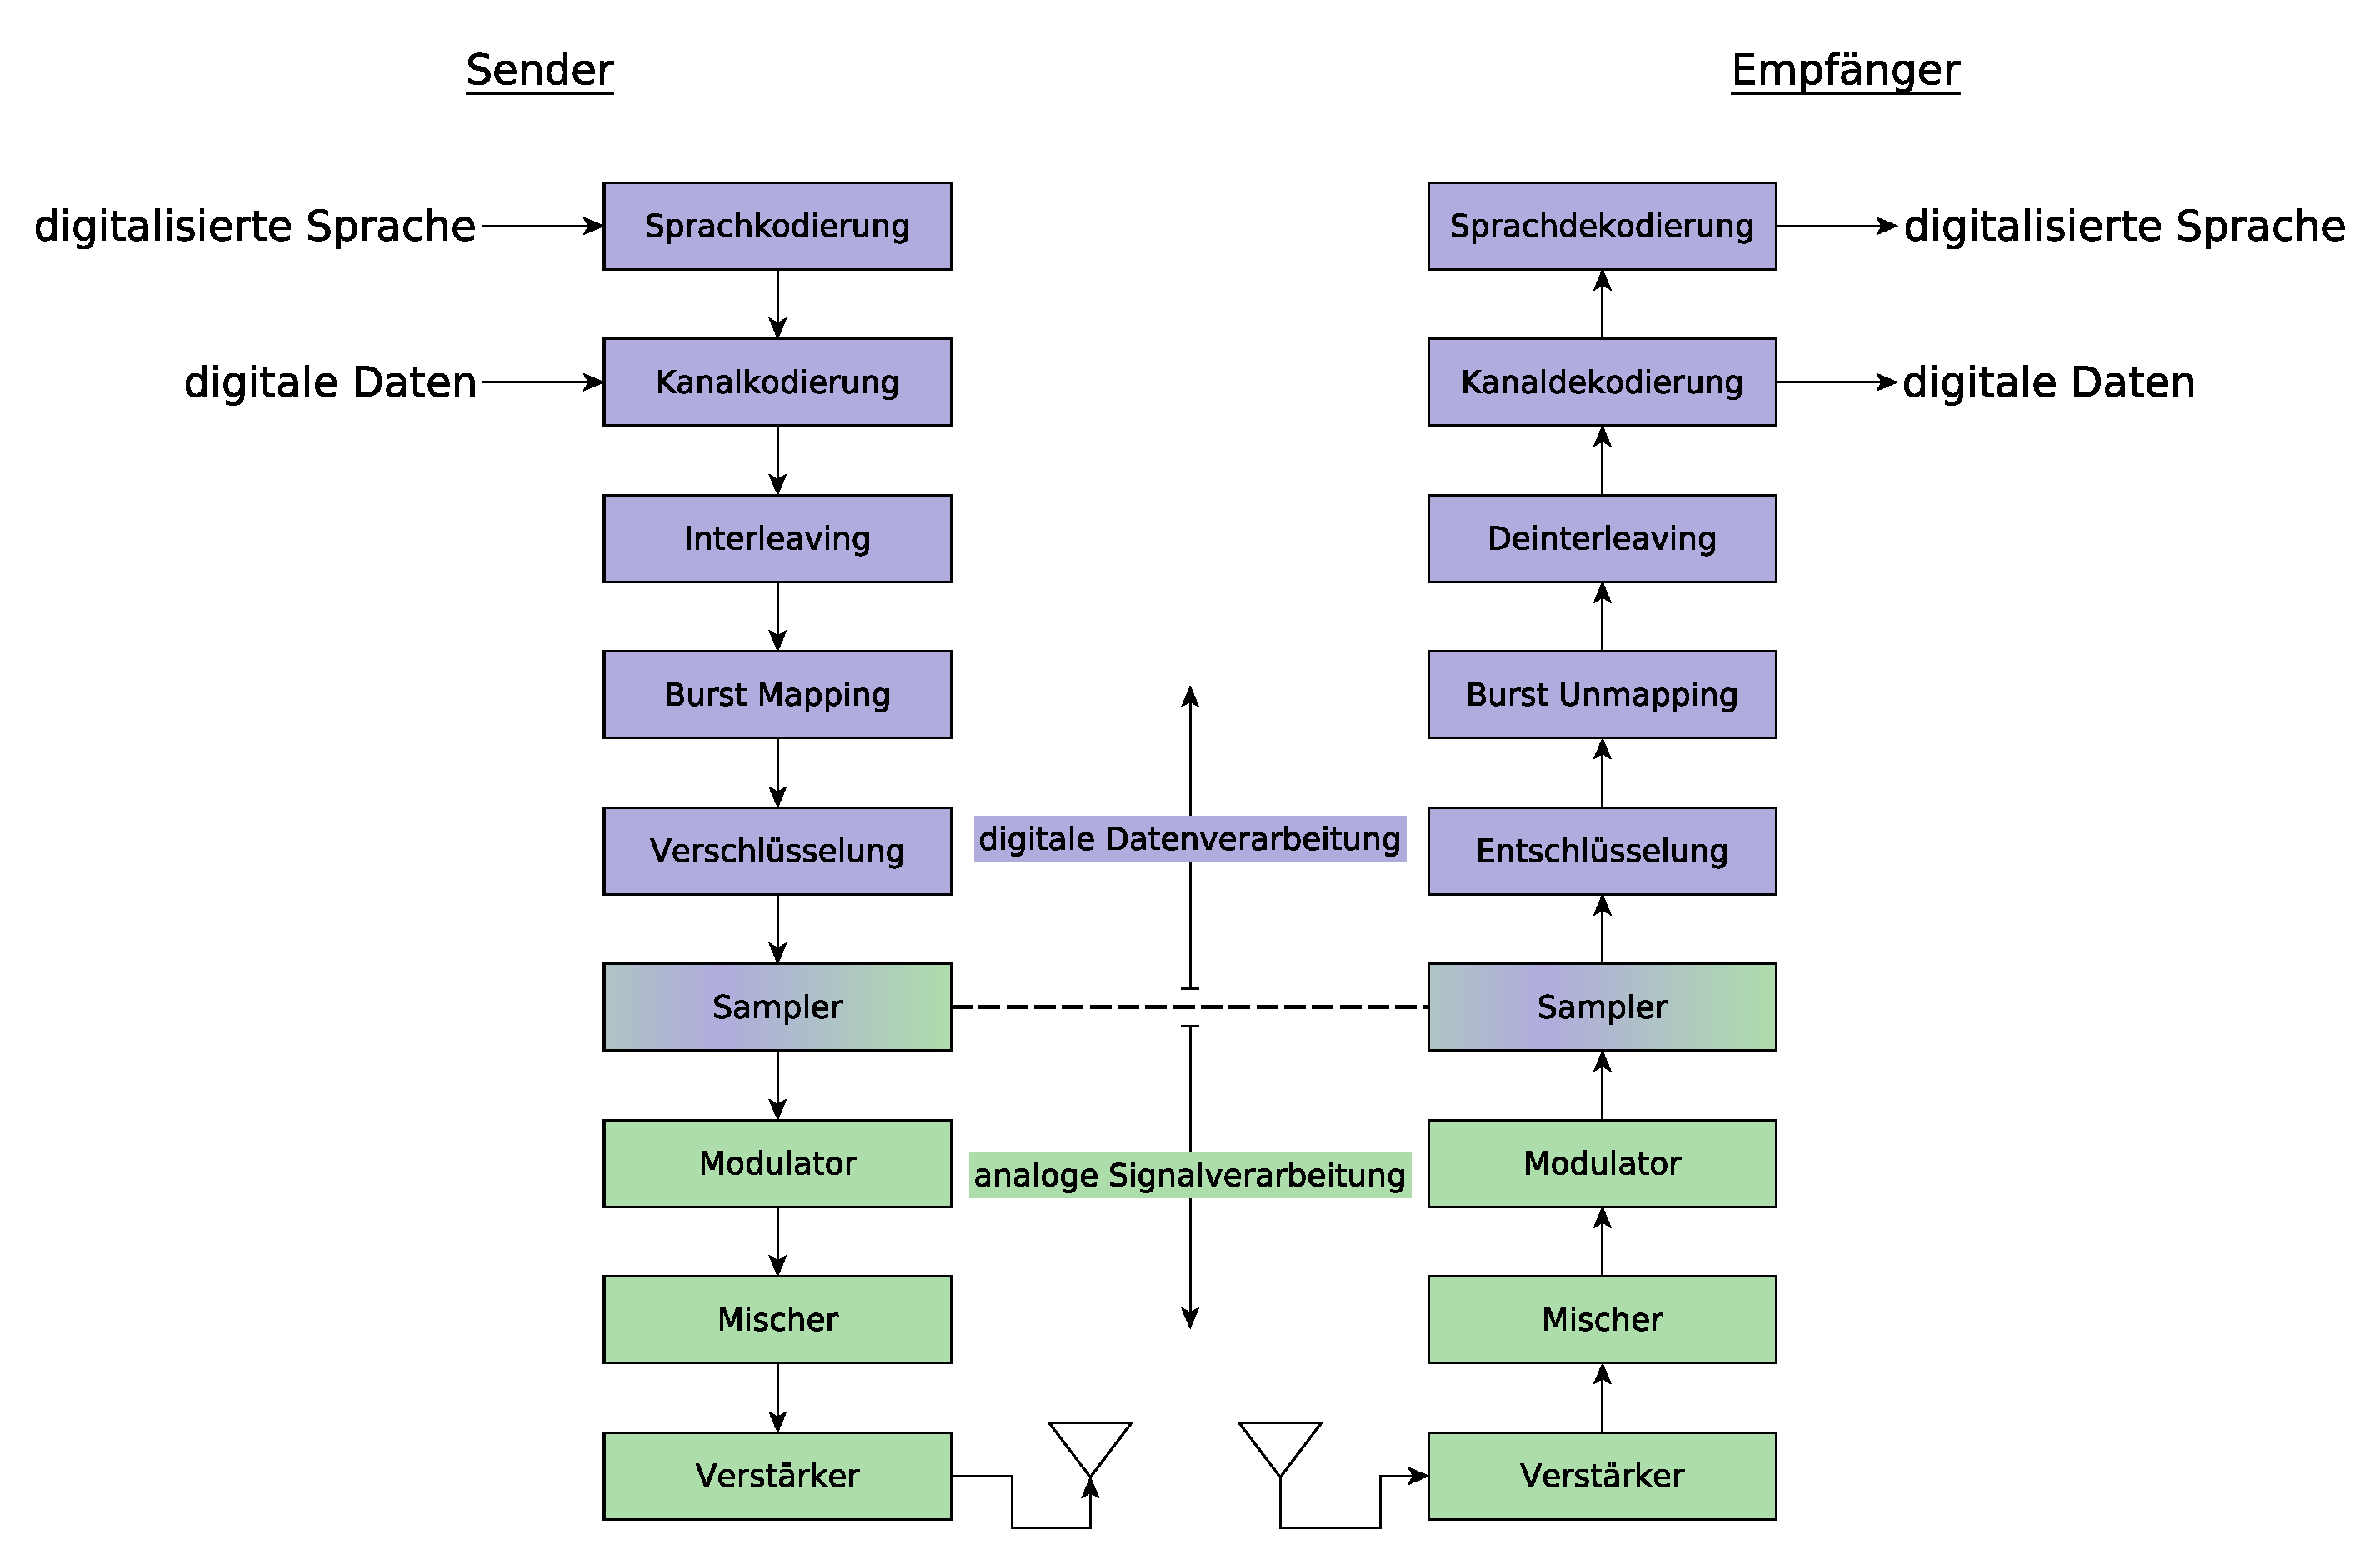
\includegraphics[width=1.0\textwidth]{figures/gsm_signal_processing.pdf}
  \end{center}
  \caption[Die Signalverarbeitung in GSM]{Die Signalverarbeitung in \ac{GSM}, erstellt mit yEd nach \citepauthor[Figure 1a]{3gpp:05.03} und \citep{zoudigital}} \label{fig:gsm-signal-processing} 
\end{figure}

Beim Sendevorgang laufen die diskreten, digitalen Daten nach Kanalkodierung und Verschlüsselung durch den Sampler, der sie in ein analoges Signal umwandelt. Dieses wird dann auf die bestehende Trägerfrequenz moduliert, gemischt und verstärkt übertragen. Beim Empfang der Daten werden die Schritte der digitalen und analogen Signalverarbeitung umgekehrt durchlaufen \citep{zoudigital}.

Aufgrund der hohen Anfälligkeit der Signalübertragung über die Luft werden Mechanismen zur Fehlererkennung und Korrektur angewandt, mit denen die Bitfehlerrate um den Faktor $10^{3}$ verringert werden kann \citep[Kap. 4.8]{eberspacher:2008:gsm-architecture}. Jeder logische Kanal hat andere Anforderungen an die übertragenen Daten. Deshalb werden, wie in \autoref{fig:0503fig1a-channel-coding} zu sehen, verschiedene Kodierungsverfahren kombiniert.

\begin{figure}[H]
  \begin{center}
    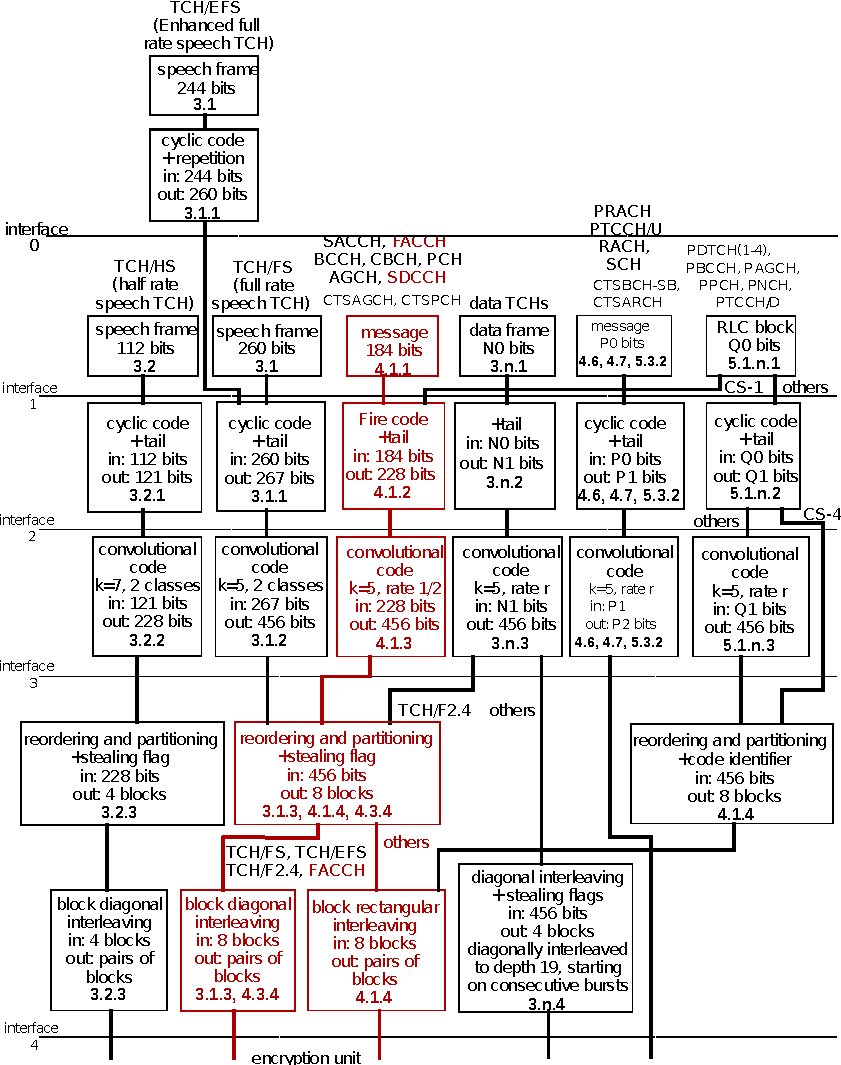
\includegraphics[width=0.9\textwidth]{figures/0503_fig_1a.pdf}
  \end{center}
  \caption[Die Kanalkodierung in GSM]{Die Kanalkodierung in \ac{GSM}, aus \citepauthor[Abb. 1a]{3gpp:05.03}} \label{fig:0503fig1a-channel-coding} 
\end{figure}

In \autoref{fig:0503fig1a-channel-coding} aus \citet{3gpp:05.03} sind die Kodierungsschritte aufgelistet, die für die verschiedenen logischen Kanäle durchlaufen werden. In jedem Kasten findet man unter dem Namen des Verfahrens die Nummer des Kapitels aus \citet{3gpp:05.03}, in dem es beschrieben wird. Die Call Setup Nachricht, die für den vorgestellten Angriff manipuliert werden muss, wird auf den Kanälen \ac{FACCH} oder \ac{SDCCH} übertragen. Die farblich markierten Verfahren sind also für die Arbeit besonders relevant und werden im Folgenden genauer erklärt.

\subsection{Blockcode}\label{hdl:blockcode}

Mit Blockcodes wird einem Block von Daten Redundanz für Fehlererkennung und/oder Fehlerkorrektur hinzugefügt. Der \ac{GSM}-Standard definiert den Einsatz von zwei Verfahren, \ac{CRC} für Nutzdatenkanäle und Firecode auf Signalisierungskanälen.

Auf Sprachkanälen werden die Informationsbits zudem in verschiedene Klassen eingeteilt, von denen nur Klasse 1 Bits besonders signifikant für die Spracherkennung sind und durch den \ac{CRC} fehlergeschützt werden. Klasse 2 Bits sind nicht so wichtig und fließen deshalb auch nicht in die Berechnung der Paritätsbits mit ein.

Für Signalisierungsnachrichten wird ein Firecode verwendet, ein linearer binärer Blockcode. Für eine Reihe von Informationsbits liefert dieser eine Anzahl redundanter Bits, die für die Fehlererkennung und -korrektur verwendet werden können. Die redundanten Bits werden durch \ac{XOR}, beziehungsweise binäre Addition der Informationsbits berechnet. 

Für alle zyklischen Codes kann die Berechnung der Redundanz als binäre Polynomdivision ausgedrückt werden. Aus der originalen Datensequenz wird ein Polynom aufgebaut, dessen Koeffizienten die Bits der Sequenz sind. Der Teiler ist ein definiertes Generatorpolynom und die Redundanz der Rest der Polynomdivision. Durch das Anhängen der Redundanz an die Datensequenz kann der Empfänger diese auf Fehler überprüfen, indem er ebenfalls durch das Generatorpolynom teilt. Ist das Ergebnis 0, sind keine Fehler aufgetreten. Es ist möglich, einen Sollrest anzugeben, der bei der Überprüfung der Datensequenz als Ergebnis herauskommen soll. Durch die \ac{XOR}-Verknüpfung der berechneten Redundanz mit dem Sollrest auf der Senderseite kommt dieser bei der Überprüfung durch den Empfänger wieder heraus. \ac{GSM} definiert als Sollrest die 40 Bits mit dem Wert 1, wodurch die Daten als fehlerfrei übertragen gelten, wenn das Ergebnis der Überprüfung \texttt{0xffffffffff} ist.
\begin{align}
&g: (x^{23} + 1) \cdot (x^{17} + x^3 + 1) = x^{40} + x^{26} + x^{23} + x^{17} + x^{3} + 1 \label{gl:firecode-gen}
\end{align}
Das Generatorpolynom (siehe \autoref{gl:firecode-gen}) des Firecodes und die Definition des Soll-Rests ist in \citetauthor[Kap. 4.1.2]{3gpp:05.03} zu finden.

Da die Eingangsdaten immer ein \ac{LAPDm} Frame sind, ist die Länge k der Informationsbits 184 Bit. Der Firecode generiert mit obigem Generatorpolynom, entsprechend dessen Grad, aus der 184 Bit langen Sequenz, 40 redundante Paritätsbits $p(k)$. In \ac{GSM} werden die berechneten Paritätsbits einfach an die Originaldaten $d(k)$ angehängt. Für die Weiterverarbeitung werden für die Faltungskodierung noch vier Nullbits angefügt, womit die ausgehenden Daten $u(k)$ die Länge von 228 Bit haben. Der Zusammenhang ist in  \autoref{eq:blockcode_2} mathematisch dargestellt.
\begin{align}\label{eq:blockcode_2}
\begin{split}
u(k) = d(k) &\quad \text{für} \, k= 0,1,...,183 \\
u(k) = p(k-184) &\quad \text{für} \, k = 184,185,...,223 \\
u(k) = 0 &\quad \text{für} \, k = 224,225,226,227
\end{split}
\end{align}
Das verwendete Generatorpolynom wurde von \citet{fire1959class} vorgestellt und bietet eine gute Erkennung und Korrektur von Fehlergruppen von bis zu 11 Bits. Obwohl eine Fehlerkorrektur möglich wäre, verzichtet \ac{GSM} darauf und verlässt sich stattdessen auf die erneute Übertragung der Nachricht, auf der von \ac{LAPDm} zur Verfügung gestellten, zuverlässigen Verbindung. In folgendem Beispiel wird der Firecode auf Testdaten angewendet.\\

%\begin{adjustbox}{max width={0.980\textwidth}, padding=3pt 2pt 3pt 0pt, frame, center}
\begin{lstlisting}[caption={[Kodierung von Testdaten mit dem Firecodes]Kodierung von Testdaten mit dem Firecodes, Datensatz generiert mit \texttt{dummycoder} (siehe \autoref{hdl:coder-impl})}, captionpos=b, language=bytetxt, numbers=none, frame=single]
Datensequenz (184 Bit):
01 20 51 03 45 04 04 60  02 00 81 5e 07 81 10 57 
81 81 81 81 15 01 01

Rest aus Polynomdivision mit Generatorpolynom (40 Bit): 
07 47 e3 10 1a

Soll-Rest in GSM (40 Bit):
ff ff ff ff ff

Paritätsbits in GSM == Rest XOR Soll-Rest (40 Bit):
f8 b8 1c ef e5

Anhängen von Paritäts- und Nullbits (228 Bit):
01 20 51 03 45 04 04 60  02 00 81 5e 07 81 10 57 
81 81 81 81 15 01 01 f8  b8 1c ef e5 0
\end{lstlisting}
%\end{adjustbox}

Blockcodes und zyklische Codes gehören zu den linearen Codes, weshalb Methoden der Linearen Algebra angewandt werden können. Für lineare Abbildungen gilt Additivität \citep[S. 142 ff.]{werner2008codierung}:
\begin{align}
\boldsymbol{u}(\boldsymbol{x} \oplus \boldsymbol{y}) = \boldsymbol{u}(\boldsymbol{x}) \oplus \boldsymbol{u}(\boldsymbol{y}) \label{gl:fire-lin}
\end{align}
Es können also die Paritätsbits berechnet werden, die bei einer Datenmanipulation kippen. Das bedeutet Blockcodes, wie der Firecode, sind nur für die Erkennung von zufälligen Fehlern ausgelegt und eignen sich nicht für den Schutz der Integrität.

\subsection{Faltungscode}\label{hdl:conv-code}

Durch Faltungskodierung, auch "`Convolutional Coding"' genannt, wird das Signal erneut mit Redundanz zur Fehlerkorrektur versehen. Wie Blockcodes lässt sich auch die Faltungskodierung polynomial beschreiben. Bei der Kodierung wird der Informationsgehalt der Eingangsbits, durch Faltung mit einer durch das Generatorpolynom definierten Maske, auf mehrere Ausgangsbits verteilt. Bei der Dekodierung kommt der Viterbi-Algorithmus zum Einsatz, der aus der kodierten Datensequenz die wahrscheinlichsten Ausgangsdaten bestimmt. Da beim Paritätscheck des Blockcodes die bereits durch den Viterbi-Dekodierer fehlerkorrigierten Daten eingehen, spricht man bei der Faltungskodierung von internem und beim Blockcode von externem Fehlerschutz \cite[Kap. 4.8.1, 4.8.2]{eberspacher:2008:gsm-architecture}.

Die Polynomdarstellung des in \ac{GSM} verwendeten "`$\nicefrac{1}{2}$ Rate Convolutional Coders"' ist in \citetauthor[Kap. 4.1.3]{3gpp:05.03} zu finden.
\begin{align}
\begin{split}
& g_0 = x^4 + x^3 + 1 \\
& g_1 = x^4 + x^3 + x + 1
\end{split}
\end{align}
Obige Gleichung bedeutet, das aus einem Eingangsbit $x$ zwei Bits $g_0$ und $g_1$ durch binäre Additionen von $x$ mit seinen Vorgängerbits generiert werden. Wo es keine Vorgängerbits gibt, werden diese als 0 definiert.

Die Eingangsdaten der Faltungskodierung sind die vom Blockcode generierte Datensequenzen. Das Ergebnis $c(k)$ der Faltungskodierung wird wie folgt als Funktion der Eingangsdaten $u(k)$ ausgedrückt:
\begin{align}\label{eq:convcode}
\begin{split}
& c(2k) = u(k-4) \oplus u(k-3) \oplus u(k) \\
& c(2k+1) = u(k-4) \oplus u(k-3) \oplus u(k-1) \oplus u(k) \quad \text{für} \, k = 0,1,...,227 \\
& u(j) = 0 \quad \forall \, j < 0
\end{split}
\end{align}\noindent
Die Faltungskodierung wird in Hardware als Schieberegister implementiert. Es wird ein Puffer von vier Bits benötigt, da die Bits bis zu vier Stellen vor dem Eingangsbit ($u(k-4)$) in die Berechnung mit eingehen. Der Puffer wird mit vier Speicherregistern realisiert. Durch die mit \ac{XOR}-Gattern implementierten Funktionen $c(2k)$ und $c(2k+1)$ werden zwei Ausgangsbits generiert. Welche Speicherregister verknüpft werden müssen, lässt sich aus \autoref{eq:convcode} ableiten. Da pro Eingangsbit zwei Ergebnisbits generiert werden, bezeichnet man den Kodierer als $\nicefrac{1}{2}$ Rate Convolutional Coder. Die vier nach dem Blockcode angehängten Nullbits sind notwendig, um das Schieberegister wieder in einen vordefinierten Zustand -- alle Register gleich 0 -- für den nächsten Block zu bringen.

\begin{figure}[H]
  \begin{center}
    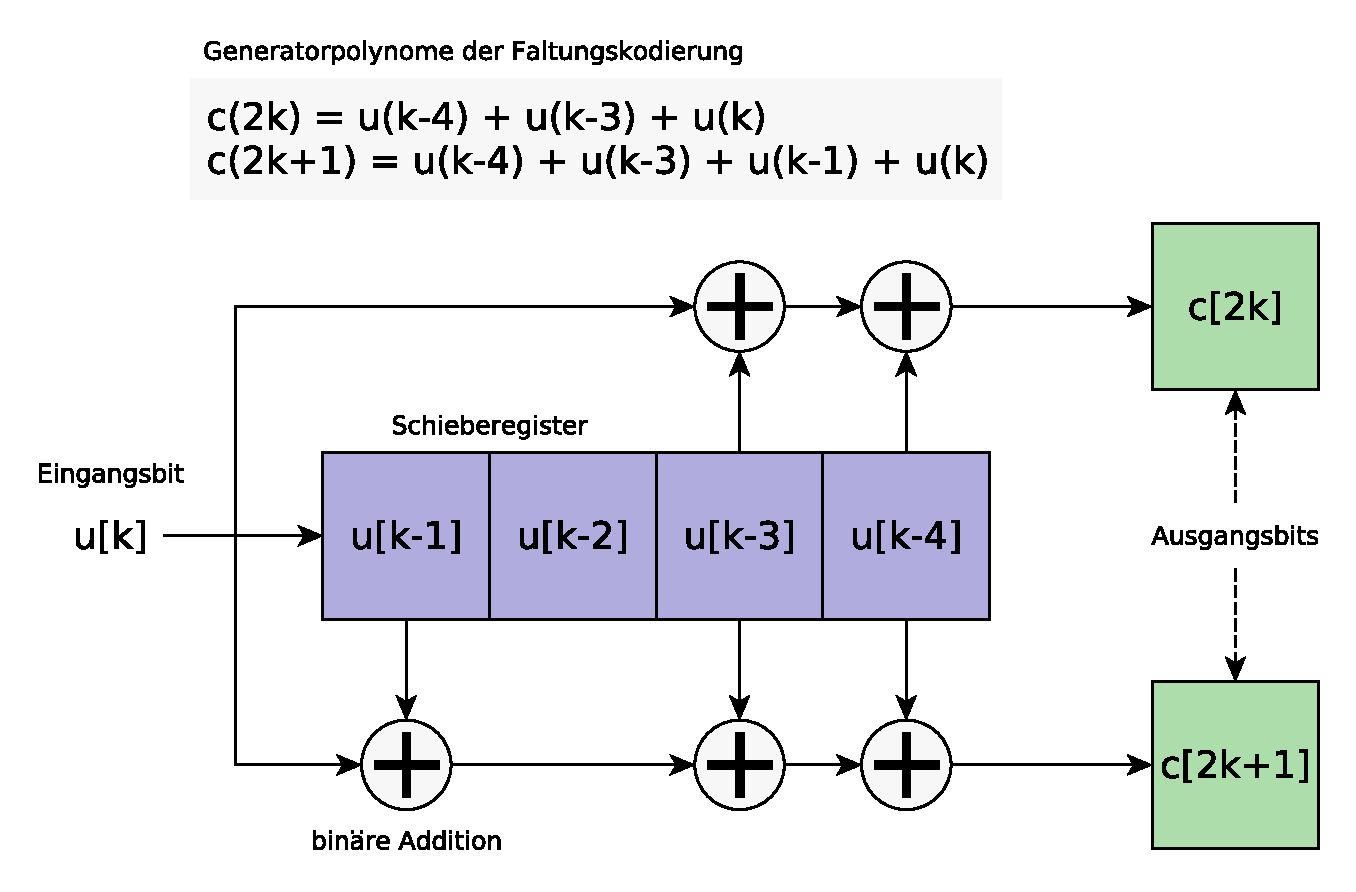
\includegraphics[width=1.0\textwidth]{figures/conv_code_shift_reg.pdf}
  \end{center}
  \caption[Das Schieberegister für die Faltungskodierung]{Das Schieberegister für die Faltungskodierung, erstellt mit yEd} \label{fig:conv_code_shift_reg} 
\end{figure}
Auf Signalisierungskanälen sind alle Datenbits wichtig und fließen in die Faltungskodierung mit ein. Bei Sprachkanälen hingegen wird ein sogenannter "`Punctured Convolutional Code"' verwendet. Um Bandbreite zu sparen werden dabei vom Kodierer nur die für die Wiederherstellung des Sprachsignals wichtigen Klasse 1 Bits kodiert, die unwichtigeren Klasse 2 Bits werden ohne Redundanz übertragen \citepauthor[Kap. 3.1.2, 3.2.2]{3gpp:05.03}. 

Wie Blockcodes gehört die Faltungskodierung zur Gruppe linearer Codes und es gilt Additivität \citep[S. 142 ff.]{werner2008codierung}:
\begin{align}
\boldsymbol{c}(\boldsymbol{x} \oplus \boldsymbol{y}) = \boldsymbol{c}(\boldsymbol{x}) \oplus \boldsymbol{c}(\boldsymbol{y})
\end{align}
In folgendem Beispiel wird die Faltungskodierung auf Testdaten angewendet.\\

%\begin{adjustbox}{max width={0.980\textwidth}, padding=3pt 2pt 3pt 0pt, frame, center}
\begin{lstlisting}[caption={[Faltungskodierung von Testdaten]Faltungskodierung von Testdaten, Datensatz generiert mit \texttt{dummycoder} (siehe \autoref{hdl:coder-impl})}, label=lst:conv_code_data, captionpos=b, language=bytetxt, numbers=none, frame=single]
Datensequenz (228 Bit):
01 20 51 03 45 04 04 60  02 00 81 5e 07 81 10 57 
81 81 81 81 15 01 01 f8  b8 1c ef e5 0

Faltungskodierte Daten (456 Bit): 
00 03 42 3c 37 bc 4f 0e  47 c7 bf 34 f0 34 c9 cc 
00 0d 3c 00 d3 c3 78 55  0c 3a 50 c3 4c 4f 37 85 
50 c3 9c c3 9c c3 9c c3  4c 78 bf 03 4f 03 a6 90 
1d 60 c3 a8 da e5 a9 3b  bf 
\end{lstlisting}
%\end{adjustbox}

\subsection{Interleaving}\label{hdl:interleaving}

Um gegen auf der Funkschnittstelle auftretende Burstfehler zu schützen, werden die Daten umsortiert und vom Interleaver verschachtelt. Blockweise Signalstörungen verteilen sich damit auf eine größere Datenmenge und können von der Fehlerkorrektur mit größerer Wahrscheinlichkeit berichtigt werden. Die aus dem Faltungskodierer kommenden Datenblöcke $N_n$ mit 456 kodierten und verschlüsselten Bits werden in Unterblöcke von je 57 Bits unterteilt. Je zwei solcher Unterblöcke werden einem Burst $B_b$ zugewiesen (siehe \autoref{fig:normal_burst}). Für Sprachkanäle wird die Stelle im Burst $B_b[j]$, an dem ein Bit eines Datenblocks $N_n[k]$ landet, in \citetauthor[Kap. 3.1.3]{3gpp:05.03} wie folgt bestimmt:
\begin{align}
\begin{split}
& i(B_b,j) = c(N_n,k) \\
& k = 0,1,...,455 \\
& n = 0,1,... \\
& b = 4 \cdot n + \left(k \bmod 8\right) \\
& j = 2 \cdot \left(\left( 49 \cdot k \right) \bmod 57 \right) + \left(\left( k \bmod 8 \right) \bdiv 4 \right)
\end{split}
\end{align}
Die Nummer des Bursts wird also durch die Nummer des Datenblocks und den Laufindex $k$ modulo $8$ auf diesem bestimmt. Das heißt jedes der acht Bits eines Bytes wird in einem anderen Burst untergebracht. Wird ein kompletter Burst fehlerhaft übertragen, erhält man auf Empfängerseite nach dem Deinterleaving die 114 fehlerhaften Bits auf einen Fehler pro Byte verteilt. So verteilte Bitfehler können von der Fehlerkorrektur berichtigt werden.

In \citetauthor[Tabelle 1]{3gpp:05.03} ist das Ergebnis von Interleaving und Umsortierung der Bits aufgelistet. Die Daten eines Blockes $N_n$ sind so auf die Bursts verteilt, dass die vorderen vier Bursts $B_{4n + 0,1,2,3}$ immer die geraden Bits [0-56] und die hinteren vier Burst $B_{4n + 4,5,6,7}$ die ungeraden Bits [57-113] enthalten. Das bedeutet, dass ein Burst immer die Daten von zwei Datenblöcken $N_n$ und $N_{n + 1}$ enthält. Die geraden Datenbits stammen aus dem höheren, die ungeraden aus dem niedrigeren Block. Diese Art der Verzahnung nennt man block-diagonales Interleaving. Alle vier Bursts beginnt ein neuer Datenblock, der in acht Bursts komplett übertragen wird. Die Übertragung einer gesamten Sprachprobe dauert somit $8 \cdot 4.615 ms = 30 ms$. Folgendes Beispiel zeigt das Ergebnis von block-diagonalem Interleaving, angewendet auf das das Ergebnis der Faltungskodierung aus \autoref{lst:conv_code_data}. Die Daten werden binär dargestellt und sind bereits ihren Bursts zugewiesen, zur besseren Kenntlichkeit sind binäre Einsen rot und Nullen blau markiert. Im Beispiel ist nur das Ergebnis des Interleaving für den Datenblock $N_n$ dargestellt, nicht die Überlagerung mit vorherigem und nachfolgenden Datenblock. So kann man erkennen, dass Bit [57-113] der ersten vier Bursts und Bit [0-56] der zweiten vier Bursts nicht befüllt sind (alle Bits gleich Null). Bit [57-113] der ersten vier Bursts wäre vom Datenblock $N_{n-1}$ befüllt worden, $N_{n+1}$ würde Bit [0-56] der zweiten vier Bursts befüllen.\\

\begin{samepage}
\begin{adjustbox}{max width={0.995\textwidth}, padding=4pt 2pt 4pt 0pt, frame, center}
\begin{lstlisting}[language=bytetxt, numbers=none]
Bit[0-56]                                                 Bit[57-113]
!!00000000000000!!@1@!!000!!@1@!!000!!@1@!!0!!@1@!!0!!@1@!!00000!!@1@!!00000!!@1@!!0!!@1@!!0!!@1@!!0!!@1@!!000!!@1@!!000!!@1@!!000!!@1@ !!000000000000000000000000000000000000000000000000000000000!! Burst 0
!!00!!@1@!!0!!@1@!!000!!@1@!!00000!!@1@!!0!!@1@!!0!!@1@!!0000000000000!!@1@!!0!!@1@!!0!!@1@!!000!!@1@!!000!!@1@!!0!!@1@!!0!!@1@!!000!!@1@!!0!!@1@!!00!! !!000000000000000000000000000000000000000000000000000000000!! Burst 1
!!00!!@1@!!0!!@1@!!000!!@1@!!0!!@1@!!0!!@1@!!0!!@1@!!000000000!!@1@!!0!!@1@!!0!!@1@!!00000000000!!@1@!!0!!@1@!!000000000!!@1@!!000!!@1@ !!000000000000000000000000000000000000000000000000000000000!! Burst 2
!!0000000000!!@1@!!0!!@1@!!0!!@1@!!000!!@1@!!000!!@1@!!0!!@1@!!0!!@1@!!0000000000000!!@1@!!0!!@1@!!0!!@1@!!0!!@1@!!0!!@1@!!00000000!! !!000000000000000000000000000000000000000000000000000000000!! Burst 3
!!000000000000000000000000000000000000000000000000000000000!! @1@!!000!!@1@!!0!!@1@!!0!!@1@!!0!!@1@!!0!!@1@!!000000000!!@1@!!0!!@1@!!0!!@1@!!0!!@1@!!000!!@1@!!000!!@1@!!0!!@1@!!00000!!@1@!!000000000000!! Burst 4
!!000000000000000000000000000000000000000000000000000000000!! @1@!!0000000!!@1@!!00000!!@1@!!0!!@1@!!0!!@1@!!000!!@1@!!0!!@1@!!000!!@1@!!00000!!@1@!!0!!@1@!!00000!!@1@!!0!!@1@!!0!!@1@!!000!!@1@!!0!!@1@!!0000!! Burst 5
!!000000000000000000000000000000000000000000000000000000000!! !!00!!@1@!!0000000!!@1@!!0!!@1@!!0!!@1@!!0!!@1@!!000!!@1@!!000!!@1@!!00000!!@1@!!0!!@1@!!0000000!!@1@!!0!!@1@!!0!!@1@!!000!!@1@!!0!!@1@!!000000!! Burst 6
!!000000000000000000000000000000000000000000000000000000000!! @1@!!0!!@1@!!0!!@1@!!000!!@1@!!00000!!@1@!!000000000!!@1@!!0!!@1@!!0!!@1@!!00000!!@1@!!0000000!!@1@!!0!!@1@!!0!!@1@!!0!!@1@!!0!!@1@!!000!!@1@!!00!! Burst 7
\end{lstlisting}
\end{adjustbox}
\begin{lstlisting}[caption={[Verschachtlung von Testdaten mit block-diagonalem Interleaving]Verschachtlung von Testdaten mit block-diagonalem Interleaving, Datensatz generiert mit \texttt{dummycoder} (siehe \autoref{hdl:coder-impl})}, basicstyle=\tiny, label=lst:interl-block-diag]
\end{lstlisting}
\end{samepage}

Das für Signalisierungskanäle angewandte Interleaving \citepauthor[Kap. 4.1.4]{3gpp:05.03} unterscheidet sich nur in der Verteilung der 57 Bit Blöcke auf die Bursts.
\begin{align}
\begin{split}
& i(B_b,j) = c(N_n,k) \\
& k = 0,1,...,455 \\
& n = 0,1,... \\
& b = 4 \cdot n + \left(k \bmod 4\right) \\
& j = 2 \cdot \left(\left( 49 \cdot k \right) \bmod 57 \right) + \left(\left( k \bmod 8 \right) \bdiv 4 \right)
\end{split}
\end{align}
Im Gegensatz zum block-diagonalen Interleaving werden die generierten Blöcke auf nur vier Bursts aufgeteilt. Es gibt keine Verzahnung von aufeinander folgenden Datenblöcken, wodurch eine Signalisierungsnachricht nach $4 \cdot 4.615 ms = 15 ms$ komplett übertragen ist. Ein Burst $B_{4n + 1,2,3,4}$ enthält also eine Kombination von geraden und ungeraden Daten des selben Datenblocks $N_n$. Das Verfahren wird deshalb block-rectangular Interleaving genannt. Die Verteilung der Bits eines Datenblocks $N_n$ auf die Burst mit block-rectangular Interleaving, ist in folgendem Beispiel dargestellt. Es werden die selbigen Eingangsdaten verwendet wie in \autoref{lst:interl-block-diag}. Anschaulich gesagt wandern Bit [57-113] der zweiten vier Bursts "`nach oben"', in die ersten vier Bursts.\\

\begin{samepage}
\begin{adjustbox}{max width={0.995\textwidth}, padding=4pt 2pt 4pt 0pt, frame, center}
\begin{lstlisting}[language=bytetxt, numbers=none]
Bit[0-56]                                                 Bit[57-113]
!!00000000000000!!@1@!!000!!@1@!!000!!@1@!!0!!@1@!!0!!@1@!!00000!!@1@!!00000!!@1@!!0!!@1@!!0!!@1@!!0!!@1@!!000!!@1@!!000!!@1@!!000!!@1@ @1@!!000!!@1@!!0!!@1@!!0!!@1@!!0!!@1@!!0!!@1@!!000000000!!@1@!!0!!@1@!!0!!@1@!!0!!@1@!!000!!@1@!!000!!@1@!!0!!@1@!!00000!!@1@!!000000000000!! Burst 0
!!00!!@1@!!0!!@1@!!000!!@1@!!00000!!@1@!!0!!@1@!!0!!@1@!!0000000000000!!@1@!!0!!@1@!!0!!@1@!!000!!@1@!!000!!@1@!!0!!@1@!!0!!@1@!!000!!@1@!!0!!@1@!!00!! @1@!!0000000!!@1@!!00000!!@1@!!0!!@1@!!0!!@1@!!000!!@1@!!0!!@1@!!000!!@1@!!00000!!@1@!!0!!@1@!!00000!!@1@!!0!!@1@!!0!!@1@!!000!!@1@!!0!!@1@!!0000!! Burst 1
!!00!!@1@!!0!!@1@!!000!!@1@!!0!!@1@!!0!!@1@!!0!!@1@!!000000000!!@1@!!0!!@1@!!0!!@1@!!00000000000!!@1@!!0!!@1@!!000000000!!@1@!!000!!@1@ !!00!!@1@!!0000000!!@1@!!0!!@1@!!0!!@1@!!0!!@1@!!000!!@1@!!000!!@1@!!00000!!@1@!!0!!@1@!!0000000!!@1@!!0!!@1@!!0!!@1@!!000!!@1@!!0!!@1@!!000000!! Burst 2
!!0000000000!!@1@!!0!!@1@!!0!!@1@!!000!!@1@!!000!!@1@!!0!!@1@!!0!!@1@!!0000000000000!!@1@!!0!!@1@!!0!!@1@!!0!!@1@!!0!!@1@!!00000000!! @1@!!0!!@1@!!0!!@1@!!000!!@1@!!00000!!@1@!!000000000!!@1@!!0!!@1@!!0!!@1@!!00000!!@1@!!0000000!!@1@!!0!!@1@!!0!!@1@!!0!!@1@!!0!!@1@!!000!!@1@!!00!! Burst 3
\end{lstlisting}
\end{adjustbox}
\begin{lstlisting}[caption={[Verschachtlung von Testdaten mit block-rectangular Interleaving]Verschachtlung von Testdaten mit block-rectangular Interleaving, Datensatz generiert mit \texttt{dummycoder} (siehe \autoref{hdl:coder-impl})}, basicstyle=\tiny]
\end{lstlisting}
\end{samepage}

\subsection{Burst Mapping}\label{hdl:burst-mapping}
Ein normaler Burst enthält zusätzlich zu den zwei 57 Bit Blöcken an Daten noch sogenannte "`Stealing Flags"' (siehe \autoref{fig:normal_burst}). Sie sind gesetzt, wenn die Daten des ihnen zugeordneten 57 Bit Blockes für die Übertragung von Signalisierungsinformationen genutzt werden. Auf Sprachkanälen kann der \ac{FACCH} somit die Bandbreite des \ac{TCH} mitbenutzen. Die Sprachdaten auf dem \ac{TCH}, die so durch Signalisierungsdaten des \ac{FACCH} ersetzt werden, werden verworfen \citepauthor[Kap. 4.3.5]{3gpp:05.03}. Der \ac{FACCH} stiehlt also Bandbreite vom \ac{TCH}, was den Namen des Flags erklärt. Auf Kanälen wie dem \ac{SDCCH}, die nur Signalisierungsinformationen übertragen, sind immer beide Flags gesetzt \citepauthor[Kap. 4.5, 4.1.5]{3gpp:05.03}.

"`Burst Mapping"' fügt in die vom Interleaving erstellten 57 Bit Blöcke Stealing Flags ein und ordnet jeweils zwei der entstandenen 58 Bit Blöcke den 116 Bit Nutzdaten eines fertigen Bursts zu. Das Beispiel zeigt die Zuordnung der schon in \autoref{hdl:interleaving} verwendeten, auf einem \ac{SDCCH} übertragenen Signalisierungsnachricht. In diesem Fall werden beide Stealing Flags gesetzt. Würde die Signalisierungsnachricht auf einem \ac{FACCH} übertragen werden, wäre sie vom Burstmapping auf acht Bursts verteilt worden. Jedem der acht Bursts würde dann nur die Hälfte seiner Nutzdaten gestohlen werden.\\

\begin{samepage}
\begin{adjustbox}{max width={0.995\textwidth}, padding=4pt 2pt 4pt 0pt, frame, center}
\begin{lstlisting}[language=bytetxt, numbers=none]
Bit[0-56]                                                     Bit[59-115]
!!00000000000000!!@1@!!000!!@1@!!000!!@1@!!0!!@1@!!0!!@1@!!00000!!@1@!!00000!!@1@!!0!!@1@!!0!!@1@!!0!!@1@!!000!!@1@!!000!!@1@!!000!!@1@ @1@ @1@ @1@!!000!!@1@!!0!!@1@!!0!!@1@!!0!!@1@!!0!!@1@!!000000000!!@1@!!0!!@1@!!0!!@1@!!0!!@1@!!000!!@1@!!000!!@1@!!0!!@1@!!00000!!@1@!!000000000000!! Burst 0
!!00!!@1@!!0!!@1@!!000!!@1@!!00000!!@1@!!0!!@1@!!0!!@1@!!0000000000000!!@1@!!0!!@1@!!0!!@1@!!000!!@1@!!000!!@1@!!0!!@1@!!0!!@1@!!000!!@1@!!0!!@1@!!00!! @1@ @1@ @1@!!0000000!!@1@!!00000!!@1@!!0!!@1@!!0!!@1@!!000!!@1@!!0!!@1@!!000!!@1@!!00000!!@1@!!0!!@1@!!00000!!@1@!!0!!@1@!!0!!@1@!!000!!@1@!!0!!@1@!!0000!! Burst 1
!!00!!@1@!!0!!@1@!!000!!@1@!!0!!@1@!!0!!@1@!!0!!@1@!!000000000!!@1@!!0!!@1@!!0!!@1@!!00000000000!!@1@!!0!!@1@!!000000000!!@1@!!000!!@1@ @1@ @1@ !!00!!@1@!!0000000!!@1@!!0!!@1@!!0!!@1@!!0!!@1@!!000!!@1@!!000!!@1@!!00000!!@1@!!0!!@1@!!0000000!!@1@!!0!!@1@!!0!!@1@!!000!!@1@!!0!!@1@!!000000!! Burst 2
!!0000000000!!@1@!!0!!@1@!!0!!@1@!!000!!@1@!!000!!@1@!!0!!@1@!!0!!@1@!!0000000000000!!@1@!!0!!@1@!!0!!@1@!!0!!@1@!!0!!@1@!!00000000!! @1@ @1@ @1@!!0!!@1@!!0!!@1@!!000!!@1@!!00000!!@1@!!000000000!!@1@!!0!!@1@!!0!!@1@!!00000!!@1@!!0000000!!@1@!!0!!@1@!!0!!@1@!!0!!@1@!!0!!@1@!!000!!@1@!!00!! Burst 3
                                                          ^ ^
                Stealing Bit [57] für Daten von Bit[0-56]  |  Stealing Bit [58] für Daten von Bit[59-115]                                                           
                                       <-----------------  |  -----------------> 
\end{lstlisting}
\end{adjustbox}
\begin{lstlisting}[caption={[Zuordnung von Testdaten zu Bursts auf dem SDCCH durch Burstmapping]Zuordnung von Testdaten zu Bursts auf dem \ac{SDCCH} durch Burstmapping, Datensatz generiert mit \texttt{dummycoder} (siehe \autoref{hdl:coder-impl})}, basicstyle=\tiny]
\end{lstlisting}
\end{samepage}

\section{Sicherheit in GSM} \label{hdl:sicherheitsmechanismen-gsm_authentifizierung}

\acused{A3}
\acused{A8}
\acused{A5}
\acused{SRES}
\acused{Ki}
\acused{RES}
\acused{RAND}
\acused{COMP128}

Da auf der Funkschnittstelle jeder Mithören kann, der ein entsprechendes Empfangsgerät besitzt, spezifiziert \ac{GSM} verschiedene Techniken und Funktionen, um den Schutz, sowie die Authentizität der Identitäten der Netzteilnehmer und die Vertraulichkeit der kommunizierten Daten zu gewährleisten. 

Die Teilnehmeridentität wird durch Verwendung einer \ac{TMSI} zur Identifikation des \ac{MS} beim Netzwerk geschützt. Ein Teilnehmer erhält vom Netzwerk diese temporäre Identifikationsnummer, die er statt seiner eindeutigen \ac{IMSI} benutzen kann, um sich für die Nutzung von Diensten beim Netzwerk zu identifizieren \citepauthor{3gpp:03.20}.

Um Authentizität von Teilnehmeridentitäten und die Vertraulichkeit von kommunizierten Nutzdaten und Signalisierungsinformationen sicherzustellen, werden in \citetauthor{3gpp:03.20} die Algorithmen \ac{A3}, \ac{A8} und \ac{A5} definiert. Eine Beschreibung der Algorithmen findet sich nicht im Standard, die Algorithmen konnten aber durch Reverse Enginnering herausgefunden werden. So veröffentlichten \citet{briceno1998implementation} die Implementierung von \ac{COMP128}, einer Kombination der \ac{A3} und \ac{A8} Algorithmen und \citet{briceno1999pedagogical} die Implementierung von A5/1 und A5/2. Mit der Entwicklung neuerer Algorithmen hat \ac{3GPP} den "`Security by Obscurity"' Ansatz fallen gelassen. So steht zum Beispiel die Spezifikation von A5/3 auf der Website von \ac{3GPP} zu Verfügung\footnote{\url{http://www.3gpp.org/specifications/60-confidentiality-algorithms}}. Die Implementierung von \ac{A3} und \ac{A8} wurde von \ac{3GPP} als netzanbieterspezifisch bezeichnet, \ac{COMP128} wäre nur eine Beispielimplementierung gewesen und war nicht für den konkreten Einsatz gedacht. A5/1 und A5/2 wurden von \ac{3GPP} auch nachträglich nicht mehr selbst veröffentlicht, finden sich aber online\footnote{\url{http://www.scard.org/gsm/}}. Die folgenden Abschnitte gehen näher auf die in \ac{GSM} verwendeten Sicherheitsalgorithmen ein.

\subsection{GSM Authentifizierung} \label{hdl:authentication}

\begin{figure}[H]
  \begin{center}
    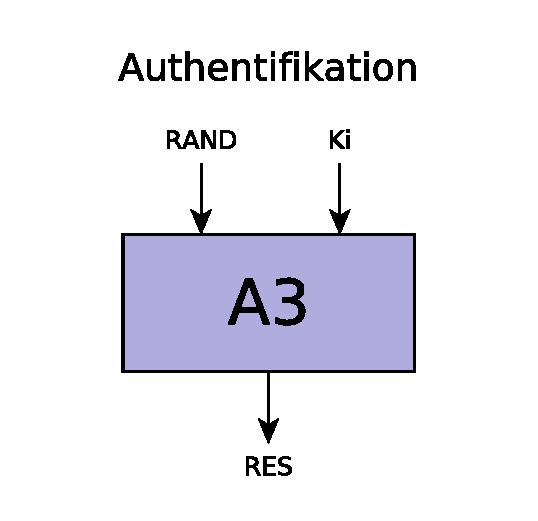
\includegraphics[width=0.5\textwidth]{figures/gsm_a3.pdf}
  \end{center}
  \caption[Der A3-Algorithmus]{Der \ac{A3}-Algorithmus, erstellt mit yEd nach \citepauthor[Abb. 3.1]{3gpp:03.20}} \label{fig:a3-algorithm}
\end{figure}

Die Authentifizierung wird vom Netzwerk gestartet. Zuerst werden vom \ac{MSC} die für die Überprüfung der Identität des Teilnehmers benötigten Werte mit seiner \ac{IMSI} beim \ac{AuC} angefragt. Das \ac{AuC} generiert die zufällige Challenge \ac{RAND} und holt sich vom \ac{HLR} den geheimen Schlüssel \ac{Ki} für die erhaltene \ac{IMSI}. Aus den beiden wird mit dem Authentifizierungsalgorithmus \ac{A8} die erwartete Antwort \ac{SRES} des Teilnehmers berechnet \citepauthor[Kap. 3, Anhang C.2]{3gpp:03.20}. Die berechneten Werte werden konkateniert und als Authentifizierungsvektor [$\ac{RAND}\parallel\ac{SRES}$] an das \ac{MSC} zurückgeschickt. Das \ac{MSC} kann der \ac{MS} nun den Authentication-Request mit der vom Netzwerk benutzten Challenge \ac{RAND} schicken. Erhält die \ac{MS} einen Authentication-Request, lässt es von der \ac{SIM}-Karte, die Zugriff auf \ac{A8} und \ac{Ki} hat, das Ergebnis \ac{RES} berechnen. Die Anfrage vom \ac{MSC} wird dann mit einer Authentication-Response, die \ac{RES} enthält, beantwortet. Ist der Vergleich $\ac{RES} == \ac{SRES}$ im \ac{MSC} erfolgreich, so ist die \ac{MS} authentifiziert.

Da das Verfahren keine gegenseitige Authentifizierung zulässt, sondern nur die des Netzteilnehmers, ermöglicht es einem Angreifer eine falschen \ac{BTS} zu installieren, dessen Identität von der \ac{MS} nicht überprüft werden kann. Durch die Einführung von gegenseitiger Authentifizierung mit dem \ac{UMTS}-\ac{AKA} und der Möglichkeit, dieses auch in \ac{GSM}-Netzwerken zu verwenden, wurde diese Schwachstelle behoben. Das Verfahren und die mögliche Interoperabilität mit 2G Infrastruktur wird in \autoref{hdl:umts-aka} erklärt.

\subsection{GSM Schlüsselgenerierung} \label{hdl:keygen}

\begin{figure}[H]
  \begin{center}
    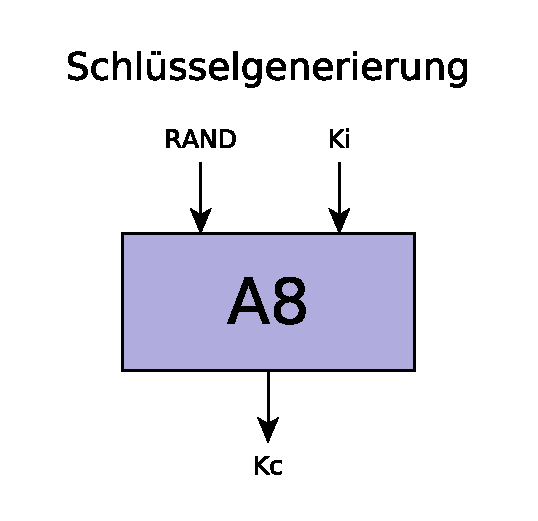
\includegraphics[width=0.5\textwidth]{figures/gsm_a8.pdf}
  \end{center}
  \caption[Der A8-Algorithmus]{Der \ac{A8}-Algorithmus, erstellt mit yEd nach \citepauthor[Abb. 4.1]{3gpp:03.20}} \label{fig:a8-algorithm}
\end{figure}

Nach erfolgreicher Authentifikation des Netzteilnehmers wird, mit dem Algorithmus \ac{A8} zur Schlüsselgenerierung, auf beiden Seiten ein 64 Bit langer \ac{Kc} berechnet, der für die weitere Verschlüsselung dieser Verbindung verwendet wird \citepauthor[Kap. 4.3, Anhang C.3]{3gpp:03.20}. Die Eingangsparameter von \ac{A8} sind die gleichen wie von \ac{A3}, vermutlich ein Grund für deren gemeinsame Implementierung in \ac{COMP128}.

Die Kombination der Verfahren zur Authentifizierung und Schlüsselgenerierung in \ac{GSM} wird \ac{AKA} genannt. Nach der Schlüsselgenerierung wird \ac{Kc} in \ac{MS} und \ac{BTS} als sogenannter Security Context unter einer \ac{CKSN} abgespeichert. Da die \ac{CKSN} bereits beim CM Service Request mitgeschickt wird, kann die \ac{BTS} prüfen, ob bereits ein gültiger Security Context mit der \ac{MS} besteht und diesen wiederverwenden. Das \ac{AKA} muss also nicht erneut ausgeführt werden, da der kryptografische Schlüssel \ac{Kc} beiden Seiten bereits bekannt ist. 

\subsection{UMTS Authentication and Key Agreement} \label{hdl:umts-aka}

\acused{K}
\acused{XMAC} 

Für \ac{UMTS} wurde mit dem 3G \ac{AKA} ein gegenseitiges Authentifizierungsverfahren spezifiziert \citepauthor{3gpp:33.102}, um die Schwachstellen der nur einseitigen 2G Authentifizierung zu beheben. Dadurch wird es einem Angreifer erschwert, in einem 3G Netzwerk eine falsche \ac{BTS} auf der \ac{Um}-Schnittstelle zu installieren, da die Authentizität des Netzwerks vom Netzteilnehmer überprüft werden kann. Außerdem wurde die Länge des zwischen 3G \ac{AuC} und \ac{USIM} geteilten geheimen Schlüssels \ac{K} von den in \ac{GSM} verwendeten 64 Bit auf 128 Bit erhöht. \autoref{fig:umts-auth-vec} zeigt die in den \ac{AUTN} einfließenden Werte und \autoref{fig:umts-auth-vec} wie die Authentifizierung des Netzwerks in der \ac{USIM} abläuft. Im \ac{UMTS}-Standard haben sich einige Bezeichnungen verändert, so wird \ac{MS} zu \ac{ME}, \ac{Ki} zu \ac{K}, und \ac{SRES} zu \ac{XRES}.

\begin{figure}[H]
  \begin{center}
    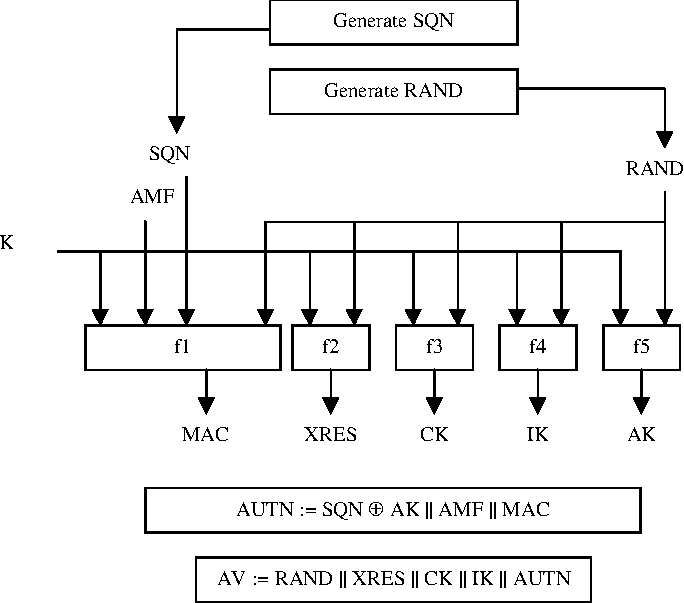
\includegraphics[width=0.7\textwidth]{figures/33102_fig_7}
  \end{center}
  \caption[Die Generierung des UMTS Authentifizierungsvektors]{Die Generierung des \ac{UMTS} Authentifizierungsvektors, aus \citepauthor[Abb. 7]{3gpp:33.102}} \label{fig:umts-auth-vec}
\end{figure}

Wie in \ac{GSM} erzeugt das \ac{AuC} zuerst eine zufällige Challenge \ac{RAND} und eine teilnehmerspezifische \ac{SQN} \citepauthor[Anhang C.1 und C.2]{3gpp:33.102}. Diese Sequenznummer bietet Schutz vor Replay-Attacken mit aufgezeichneten Authentifizierungsabläufen, da das \ac{ME} nur Anfragen akzeptiert, deren \ac{SQN} ungefähr gleich der im \ac{ME} mitgezählten \ac{SQN} ist. Ein proprietäres \ac{AMF} geht ebenfalls in die Berechnung mit ein \citepauthor[Anhang H]{3gpp:33.102}.
Das \ac{AuC} erzeugt dann folgende Werte:
\begin{itemize}
\item \textbf{\acf{MAC}}: $MAC = f1_K (SQN \parallel RAND \parallel AMF)$ 
\item \textbf{\acf{XRES}}: $XRES = f2_K (RAND)$ wobei f1 und f2 Authentifizierungsfunktionen sind.
\item \textbf{\acf{CK}}: $CK = f3_K (RAND)$
\item \textbf{\acf{IK}}: $IK = f4_K (RAND)$
\item \textbf{\acf{AK}}: $AK = f5_K (RAND)$ wobei f3, f4 und f5 Schlüsselerzeugungsfunktionen sind. \ac{AK} wird benutzt um die Sequenznummer zu anonymisieren und kann auch 0 sein, wenn das nicht erforderlich ist.
\end{itemize}
Aus diesen wird schließlich der Authentifizierungsvektor $\ac{AUTN} = \ac{SQN} \oplus \ac{AK} \parallel \ac{AMF} \parallel \ac{MAC}$ gebildet und im Authentication-Request an den Mobilfunkteilnehmer ausgeliefert.

\begin{figure}[H]
  \begin{center}
    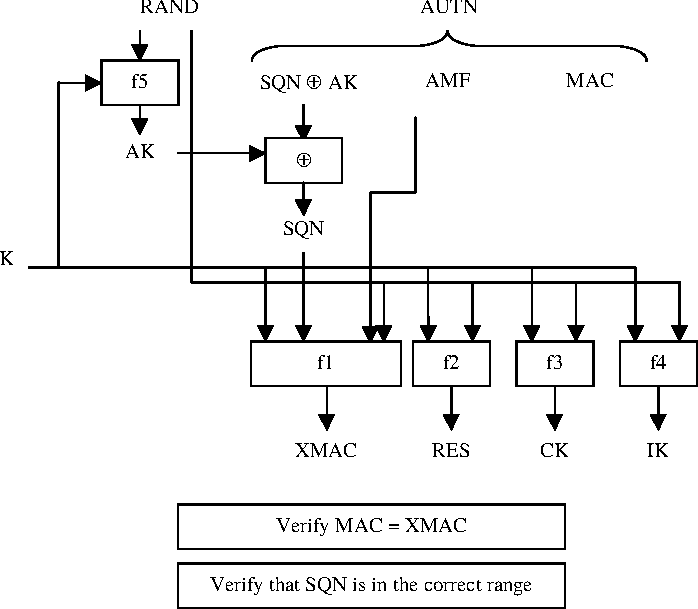
\includegraphics[width=0.7\textwidth]{figures/33102_fig_9}
  \end{center}
  \caption[Die Authentifizierung des Netzwerks in der USIM]{Die Authentifizierung des Netzwerks in der \ac{USIM}, aus \citepauthor[Abb. 9]{3gpp:33.102}} \label{fig:auth-in-usim}
\end{figure}

Erhält das \ac{ME} den Authentication-Request des Netzwerks, so kann es mit der \ac{AUTN} überprüfen, ob dieses Kenntnis seines geheimen Schlüssels \ac{K} hat. 

Als erstes löst es die Anonymisierung der Sequenznummer auf und holt sich deren Wert mit $\ac{SQN} = (\ac{SQN} \oplus \ac{AK}) \oplus \ac{AK}$, wobei für die Berechnung von \ac{AK} die Funktion f5, die auch dem \ac{AuC} zur Verfügung steht, benutzt wird. Sollte die erhaltene \ac{SQN} nicht innerhalb der richtigen Größenordnung liegen, wird ein Synchronisationsfehler mit der aktuellen \ac{SQN} der \ac{USIM} an das Netzwerk zurückgeschickt und die laufende Authentifizierung abgebrochen.

Mit der Sequenznummer und \ac{AMF} kann nun aus dem \ac{AUTN} der erwartete Authentifizierungscode des Netzwerks \ac{XMAC} berechnet werden. Wenn dieser gleich dem aus \ac{AUTN} erhaltenen \ac{MAC} ist, weiß die \ac{USIM}, dass das Netzwerk ebenfalls den geheimen Schlüssel \ac{K} kennt. Das Netzwerk ist somit authentifiziert und die Authentication-Response mit dem Ergebnis \ac{RES} wird zurückgeschickt. Die anschließende Authentifizierung der Netzteilnehmer läuft wie in \ac{GSM} durch die Überprüfung \ac{RES} == \ac{XRES} des Netzwerks.

Der Schlüssel \ac{CK} geht dann in den Verschlüsselungsalgorithmus ein und sorgt wie schon in \ac{GSM}, für Vertraulichkeit der Daten. \ac{IK} ist in 3G neu und wird verwendet, um mit der Integritätsfunktion f9 \citepauthor[Kap. 6.5.3]{3gpp:33.102} die Integrität der Daten sicherzustellen.

Das für \ac{UMTS} spezifizierte \ac{AKA} kann in \ac{GSM} ebenfalls benutzt werden, sofern der Netzteilnehmer und das \ac{AuC} die 3G Authentifizierungsverfahren unterstützen. \autoref{fig:3g-aka-in-2g} zeigt die verschiedenen Möglichkeiten der Interoperabilität zwischen 2G und 3G Netzwerk- und \ac{ME}. Da aktuelle \acp{ME} (Mobilfunkgeräte, \ac{USIM}) und Kernnetzwerke (\ac{AuC}) alle 3G kompatibel sind, wird das \ac{GSM}-\ac{AKA} in der Regel nicht mehr benutzt.

\begin{figure}[H]
  \begin{center}
    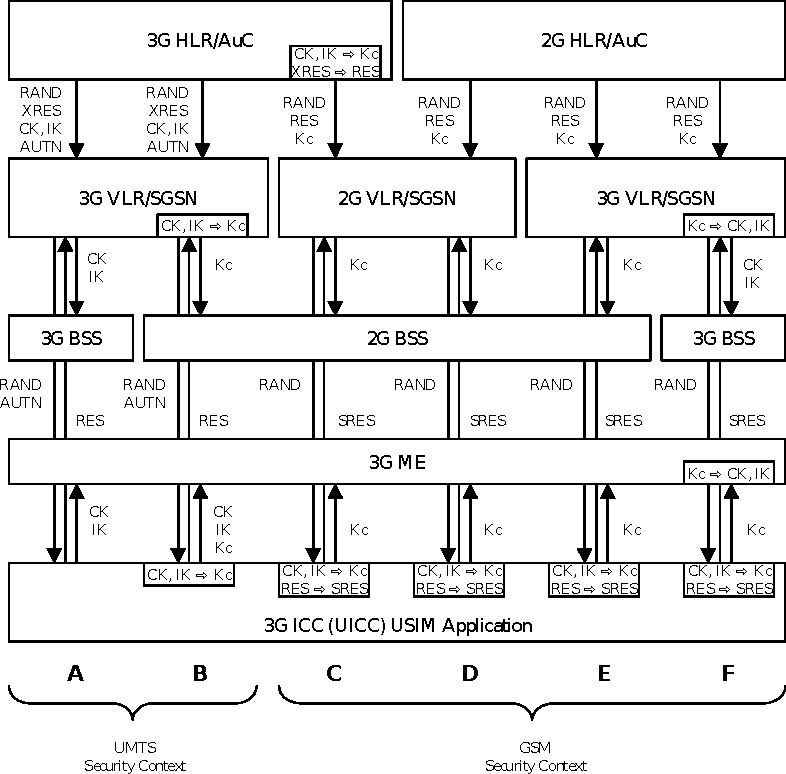
\includegraphics[width=0.8\textwidth]{figures/31900_fig_1}
  \end{center}
  \caption[Interoperabilität des 3G AKA mit 2G Netzwerken]{Interoperabilität des 3G \ac{AKA} mit 2G Netzwerken, aus \citepauthor[Abb. 1]{3gpp:31.900}} \label{fig:3g-aka-in-2g}
\end{figure}

Die Verwendung des \ac{UMTS}-AKA in 2G Netzwerken basiert darauf, dass das \ac{MSC} den vom \ac{AuC} erhaltenen Wert (\ac{RAND} oder \ac{AUTN}) einfach nur in den Authentication-Request einfügt und weiterleitet und \ac{SRES} nicht selbst berechnet. Von einem 3G-fähigen \ac{AuC} erhält die \ac{USIM} also den Wert von \ac{AUTN}, mit dem sie das Netzwerk authentifizieren kann. Für die Authentication-Response muss die \ac{USIM} die korrekte Antwort \ac{RES} berechnen mit der sie, wie im 2G Standard definiert, im \ac{MSC} authentifiziert wird. Die einzigen Komponenten, die für die Ausführung des \ac{UMTS}-\ac{AKA} 3G-fähig sein müssen, sind also \ac{USIM} und \ac{AuC}. Der von f3 berechnete kryptografische Schlüssel \ac{CK} wird von der 2G \ac{BTS} als \ac{Kc} verwendet. Für den Integritätsschlüssel \ac{IK} hat die \ac{BTS} aber keine Verwendung. Die Integrität der übertragenen Daten bleibt weiterhin ungeschützt.

\subsection{Verschlüsselung} \label{hdl:ciphering}

Bevor die Kommunikation über die Funkschnittstelle verschlüsselt werden kann, muss der verwendete \ac{A5}-Algorithmus zwischen \ac{MS} und \ac{BTS} ausgehandelt werden \citepauthor[Kap. 4.8]{3gpp:03.20}, was in der "`\ac{MM} Connection Establishment Prozedur"' \citepauthor[Kap. 4.5.1.1]{3gpp:24.008} genau beschrieben wird. Die \ac{A5}-Algorithmen sind in der Hardware von Endgerät und \ac{BTS} realisiert, da sie in Echtzeit verschlüsseln und entschlüsseln müssen.

\begin{figure}[H]
  \begin{center}
    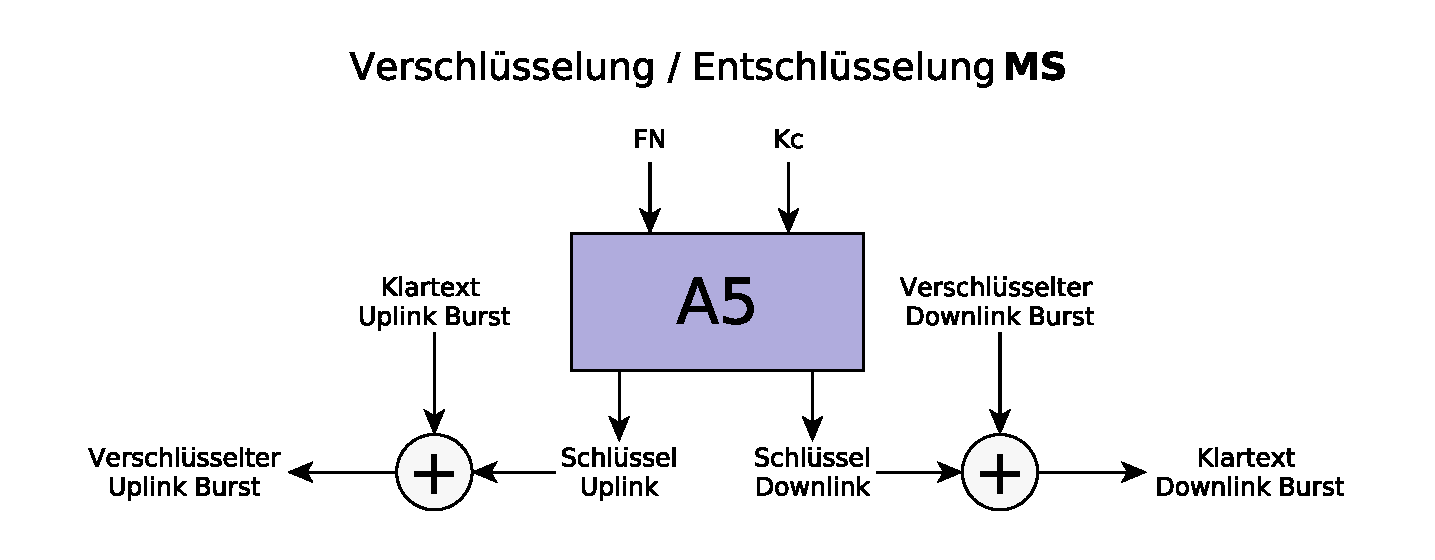
\includegraphics[width=1.0\textwidth]{figures/gsm_a5.pdf}
  \end{center}
  \caption[Der A5-Algorithmus]{Der \ac{A5}-Algorithmus, erstellt mit yEd nach \citepauthor[Abb. C.2]{3gpp:03.20}} \label{fig:a5-algorithm}
\end{figure}

Die \ac{MS} schickt der \ac{BTS} im \ac{CM} Service Request \citepauthor[Kap. 10.5.1.6]{3gpp:24.008} unter anderem das Mobile Station Classmark 2, welches ihre unterstützten Verschlüsselungsverfahren enthält. Die \ac{BTS} wählt daraus den größten gemeinsamen Nenner aus und informiert die \ac{MS} im \ac{CM} Service Accept \citepauthor[Kap. 9.2.5]{3gpp:24.008} über diesen. Durch die ebenfalls im Request übertragene \ac{CKSN} kann das Netzwerk überprüfen, ob schon ein übereinstimmender Security Context zwischen \ac{MS} und Netzwerk besteht, oder erst durch die Authentifizierung des Teilnehmers erstellt werden muss. Ist der beste gemeinsam verfügbare Algorithmus gefunden und \ac{Kc} bekannt, kann die Verbindung mit diesem geschützt werden. Die \ac{FN}, die mit in die Schlüsselstromgenerierung einfließt, verhindert Replay-Angriffe. Da diese nach einem Hyperframe allerdings wieder bei 0 beginnt und zumindest in einem laufenden Gespräch kein neuer Security Context zwischen \ac{MS} und \ac{BTS} ausgehandelt wird, wiederholt sich etwa alle drei Stunden und 26 Minuten der verwendete Schlüsselstrom. Für ein Gespräch, welches länger dauert entsteht dadurch ein Sicherheitsproblem, da der Schlüsselstrom wiederverwendet wird.
\begin{align}\label{eq:key-stream-reuse_1}
\begin{split}
&(A \oplus C) \oplus (B \oplus C) = (A \oplus B) \oplus (C \oplus C) = A \oplus B \\
\end{split}
\end{align}\noindent
\autoref{eq:key-stream-reuse_1} zeigt, dass bei Verwendung des gleichen Schlüsselstroms C für zwei verschiedene Klartextdatenströme A und B, deren \ac{XOR}-Kombination herausgefunden werden.
\begin{align}\label{eq:key-stream-reuse_2}
\begin{split}
&\text{A bekannt} \Rightarrow A \oplus A \oplus B  = B \\
&\text{B bekannt} \Rightarrow B \oplus B \oplus A = A 
\end{split}
\end{align}
Es gibt verschiedene Ansätze und Möglichkeiten, die Datenströme wieder voneinander zu trennen \citep[Kap. 3]{borisov2001intercepting}. \autoref{eq:key-stream-reuse_2} zeigt die Idee dahinter. Aus bekannten Teilen von A kann direkt der Inhalt dieses Teils von B hergeleitet werden und umgekehrt. 

Alle \ac{A5} Verschlüsselungsverfahren sind Stromchiffren und basieren auf der binären Addition des Datenstroms mit einem generierten Schlüsselstrom. In Anhang, in \autoref{hdl:a_a5} werden die von \ac{3GPP} für \ac{GSM} spezifizierten \ac{A5}-Verschlüsselungsverfahren kurz aufgeführt.

Laut Untersuchungen von \citet{gsmmap:secrep-ger} werden in deutschen 2G Netzen aktuell nur die Algorithmen A5/1 und A5/3 unterstützt. Dabei hat A5/1 bekannte Schwachstellen und A5/3 eine geringe Schlüssellänge die ihn verwundbar für Bruteforce Angriffe macht. Der aktuell (Stand 2017) als sicher geltende Algorithmus A5/4 \citep{3gpp:55.226} ist zwar seit einigen Jahren spezifiziert, wird aber nicht verwendet.

\begin{table}[H]
\centering
\begin{tabular}{|l|l|l|l|l|}
\rowcolor[HTML]{F7F7F7}
\hline
              & \textbf{O2} & \textbf{Eplus} & \textbf{Vodafone} & \textbf{Telekom} \\ \hline
\textbf{A5/1} & 73\%        & 56\%           & 41\%              & 26\%             \\ \hline
\textbf{A5/3} & 27\%        & 44\%           & 59\%              & 74\%             \\ \hline
\end{tabular}
\caption[Die prozentuale Verteilung der A5-Algorithmen in Deutschland]{Die prozentuale Verteilung der \ac{A5}-Algorithmen in Deutschland, aus \citep{gsmmap:secrep-ger}} \label{a5-usage-germany}
\end{table}

\subsection{Zusammenspiel der Sicherheitsalgorithmen in GSM}

\autoref{fig:encryption-overview} stellt das Zusammenspiel der Sicherheitsalgorithmen in \ac{GSM} dar. Aus \ac{Ki} und der im \ac{AKA} erhaltenen Challenge \ac{RAND}, berechnet das \ac{MS} mit \ac{A3} das Ergebnis \ac{RES} und schickt es an das Netzwerk zurück. Das Netzwerk vergleicht das Ergebnis des \ac{MS} mit dem eigenen als Authentizitätsprüfung. Aus den gleichen Eingangsparametern berechnet \ac{A8} auf beiden Seiten den Schlüssel \ac{Kc}. Nach erfolgreicher Authentifizierung und Aktivierung der Verschlüsselung wird aus \ac{Kc} und der aktuellen \ac{FN} der Schlüsselstrom für Uplink und Downlink generiert. Durch die \ac{XOR}-Verknüpfung mit den 114 verschlüsselten Nutzdatenbits eines dekodierten, eingehenden Burst kann dieser entschlüsselt werden. Durch die Verknüpfung mit dem unverschlüsselten Nutzdatenbits eines ausgehenden Bursts wird dieser verschlüsselt.

\begin{figure}[H]
  \begin{center}
    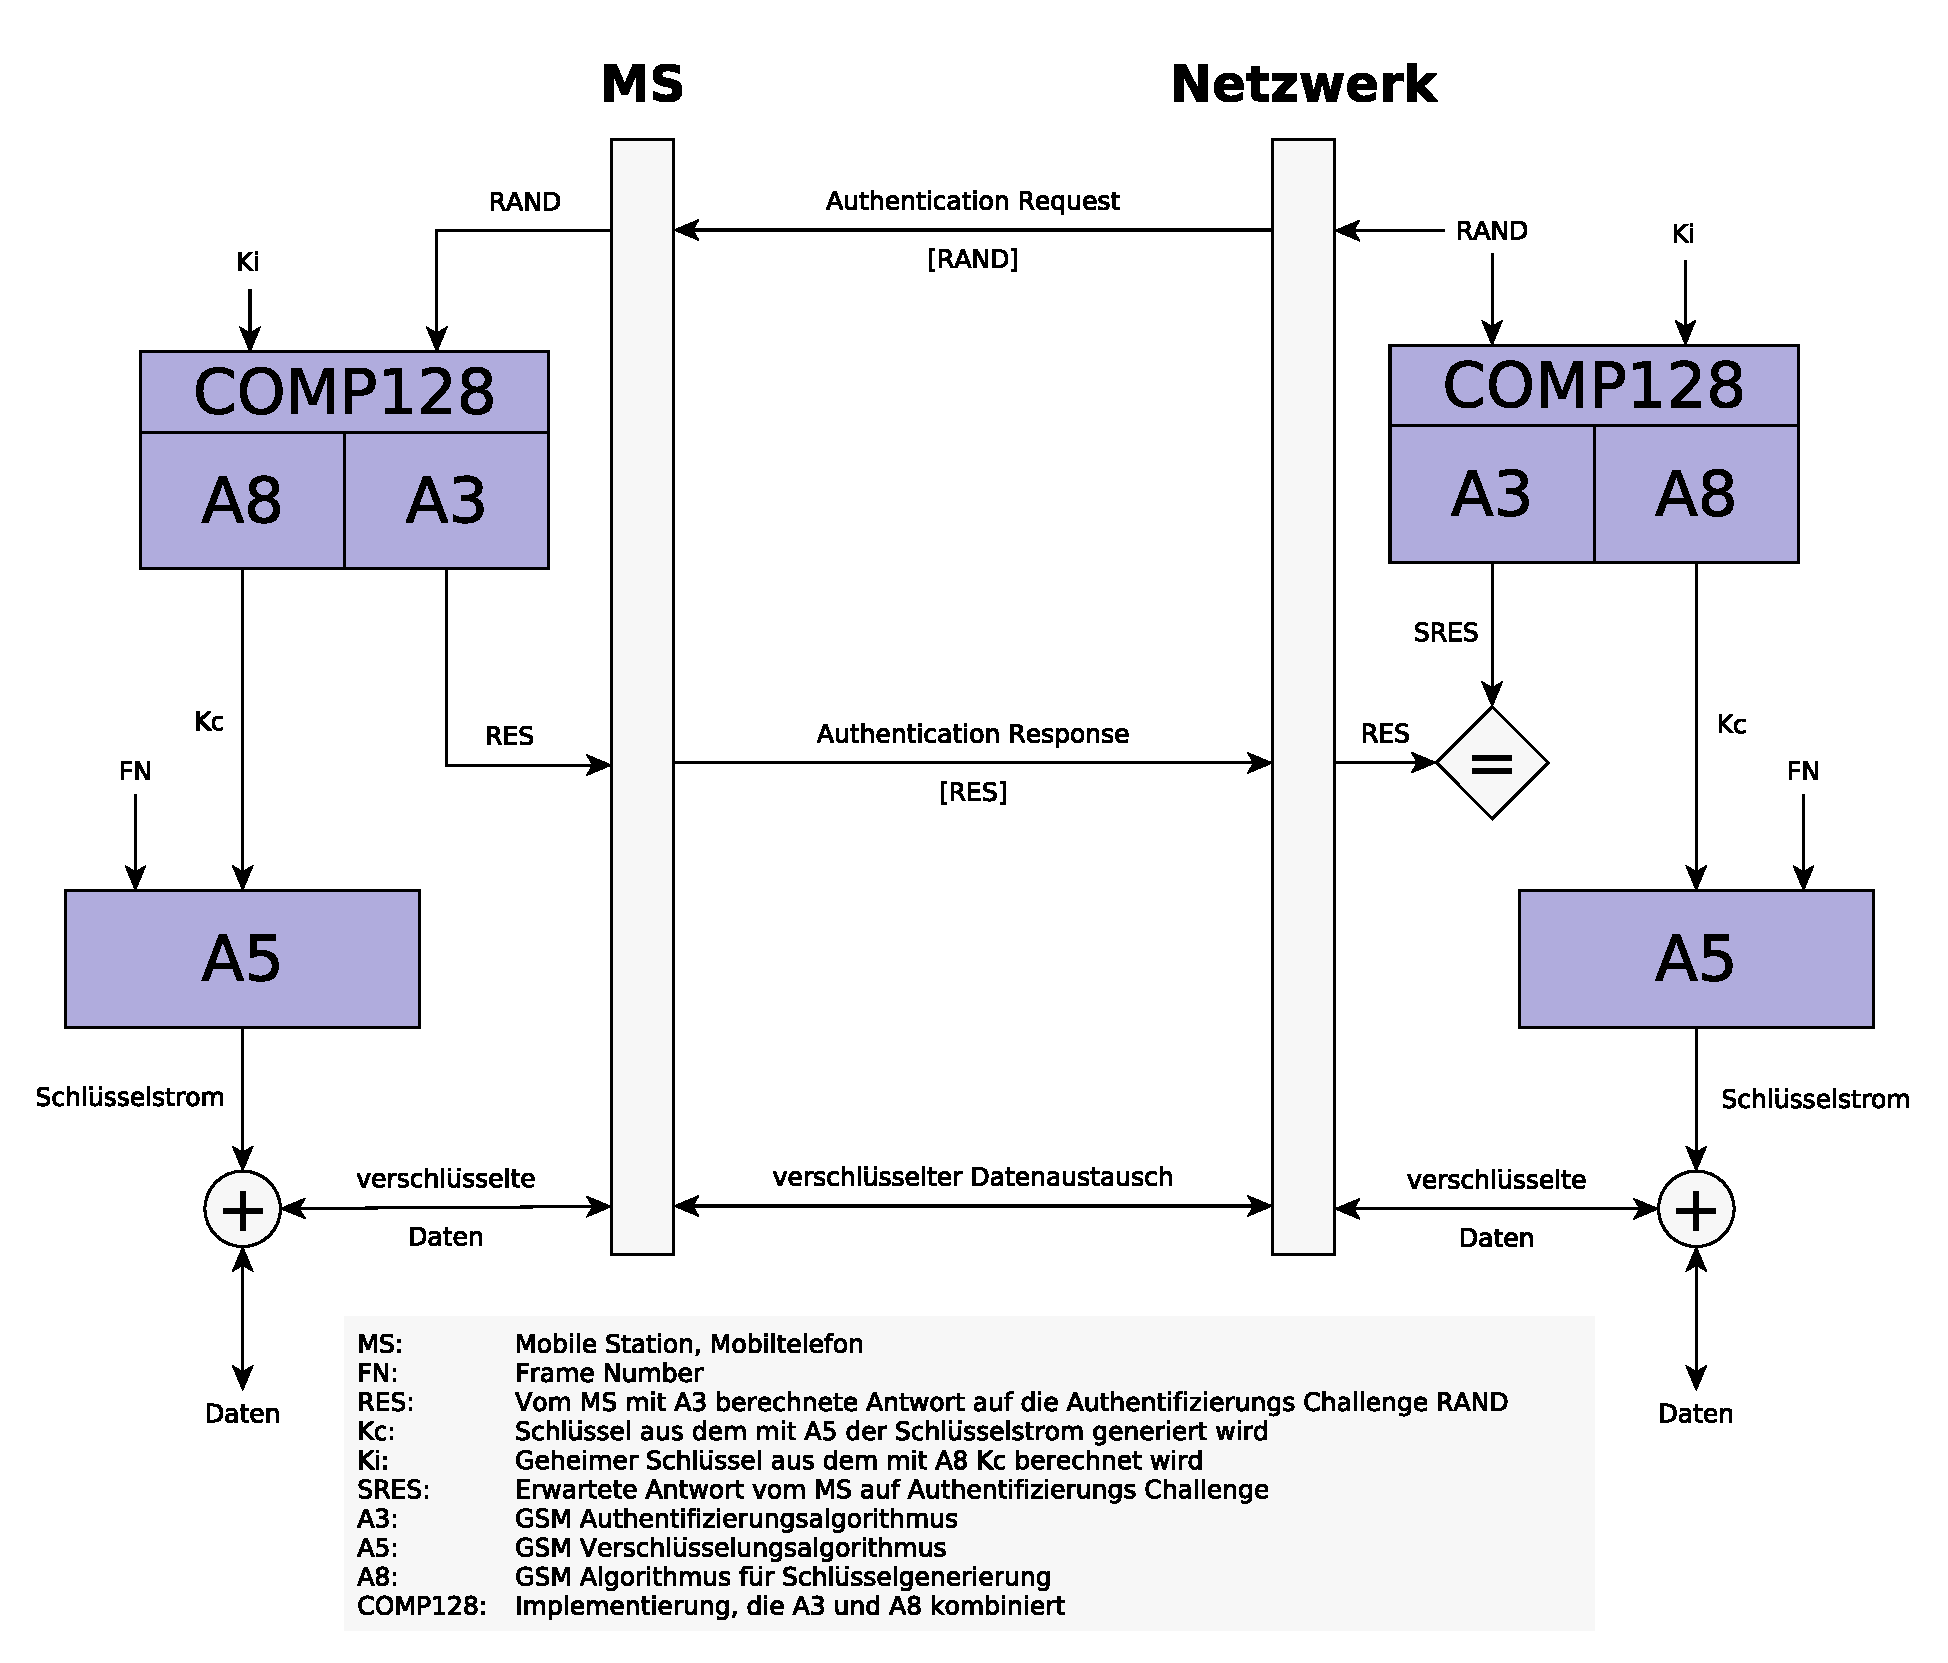
\includegraphics[width=1.0\textwidth]{figures/gsm_security_overview.pdf}
  \end{center}
  \caption[Das Zusammenspiel der GSM Sicherheitsalgorithmen]{Das Zusammenspiel der \ac{GSM} Sicherheitsalgorithmen, erstellt mit yEd} \label{fig:encryption-overview}
\end{figure}

\section{Timing Advance}\label{hdl:ta}

Da die Datenübertragung, abhängig von der Entfernung zwischen \ac{MS} und \ac{BTS}, unterschiedlich lange dauert, muss regelmäßig die Signallaufzeit gemessen und daraus der \ac{TA}-Wert \citepauthor[Kap. 6.1]{3gpp:04.04} berechnet werden. Dieser bestimmt, wie viel früher die \ac{MS} ihre Daten losschicken muss, damit sie zum richtigen Zeitpunkt bei der \ac{BTS} ankommen. Wird kein Timing-Advance verwendet, stimmt der Zeitpunkt der Ankunft des Signals unter Umständen nicht mit dem Anfang eines \ac{TDMA}-Zeitschlitzes überein. Damit liegt die Nachricht außerhalb eines gültigen physikalischen und logischen Kanals und kann von der \ac{BTS} nicht richtig dekodiert werden. Auf der Seite des \ac{MS} wird die zeitliche Verzögerung bei der Synchronisation mit der \ac{BTS} berücksichtigt, weshalb dort die Nachrichten in den korrekten Zeitschlitzen ankommen.

Der erste \ac{TA}-Wert wird dem \ac{MS} in der "`Immediate Assignment"' Nachricht auf dem \ac{AGCH} mitgeteilt und während einer Verbindung auf dem \ac{SACCH} aktualisiert. Der \ac{TA}-Wert ist quantisiert durch Vielfache der Bitübertragungsdauer von $3,7\mu s$. Er kann Werte zwischen 0 und 63 annehmen, wodurch sich der Sendezeitpunkt maximal um $63 \cdot 3.7\mu = 233\mu s$ verschieben lässt. Das entspricht etwas weniger als einem halben Burst. Das elektromagnetische Funksignal breitet sich mit Lichtgeschwindigkeit aus. In der Zeit von $233\mu s$ wird also ein Weg von ca. $300.000 \nicefrac{km}{s} \cdot 233 \cdot 10^{-6} s = 69.9 km$ zurückgelegt, womit sich ein maximaler Abstand vom \ac{MS} zur \ac{BTS} von etwa $35km$ realisieren lässt.